\documentclass{rmutt-project-thai}

\title{ชื่อโครงงานภาษาไทย}
\engtitle{Title of the Project}
\year{2567}
\firststudent{นางสาวช่ื่อนักศึกษา นามสกุลนักศึกษา}
\firststudentid{11590900001}
\secondstudent{นายช่ื่อนักศึกษา นามสกุลนักศึกษา}
\secondstudentid{11590900002}
%\thirdstudent{นายช่ื่อนักศึกษา นามสกุลนักศึกษา}
%\thirdstudentid{11590900002}

\advisor{ศ. ดร.ชื่ออาจารย์ นามสกุลอาจารย์}
\coadvisor{ศ. ดร.ชื่ออาจารย์ นามสกุลอาจารย์}
%\extadvisor{ศ. ดร.ชื่ออาจารย์ นามสกุลอาจารย์}


\begin{document}
%-------------------
\makecover
%-------------------
\approval
\par\bigskip
\headcommittee{Prof. Dr. Name Surname}
\\[4em]\par\noindent
The project committee includes the following.
\committee{Prof. Dr. Name Surname}{Advisor}
\committee{Prof. Dr. Name Surname}{Advisor}
\committee{Prof. Dr. Name Surname}{Committee}
\committee{Prof. Dr. Name Surname}{Committee}
\committee{Prof. Dr. Name Surname}{Committee}

\abstract{
%Thai
เทคโนโลยีวิสัยทัศน์วาทกรรมพันธกิจพลเมืองนวัตกรรม ล้ำสมัยสุขภาวะสตาร์ทอัพคุณธรรมสนธิกำลังประชา 
เอสเอ็มอีก้าวหน้าผสมผสานจริยธรรมคุณธรรมระดับสากลบริหาร การลงทุนบริหารวาทกรรมเอสเอ็มอีจริยธรรมโลกาภิวัฒน์คุณธรรมสร้างสรรค์สนธิกำลัง 
มุ่งมั่นพัฒนาล้ำสมัยสุขภาวะลงทุนเป้าหมาย สร้างสรรค์สนธิกำลังจัดการบูรณาการสุขภาวะพัฒนาสตาร์ทอัพ 
วิสาหกิจจริยธรรมลงทุนเอสเอ็มอีเป้าหมายจัดการพันธกิจ อาเซียนพลเมืองเป้าหมายวาทกรรมก้าวหน้าลงทุนคุณธรรมสร้างสรรค์มุ่งมั่น 


เทคโนโลยีวิสัยทัศน์วาทกรรมพันธกิจพลเมืองนวัตกรรม ล้ำสมัยสุขภาวะสตาร์ทอัพคุณธรรมสนธิกำลังประชา 
เอสเอ็มอีก้าวหน้าผสมผสานจริยธรรมคุณธรรมระดับสากลบริหาร การลงทุนบริหารวาทกรรมเอสเอ็มอีจริยธรรม โลกาภิวัฒน์คุณธรรม 
มุ่งมั่นพัฒนาล้ำสมัยสุขภาวะลงทุนเป้าหมาย สร้างสรรค์สนธิกำลังจัดการบูรณาการสุขภาวะพัฒนาสตาร์ทอัพ 
}{
%Keywords-Thai
เทคโนโลยี, วิสัยทัศน์, วาทกรรม, พันธกิจ, นวัตกรรม
}{
%English
Lorem ipsum dolor sit amet, consectetur adipiscing elit. Maecenas finibus blandit mauris et pharetra. Praesent sed accumsan enim, id facilisis felis. 
Sed sodales euismod sollicitudin. Sed aliquam purus eu ultricies semper. 
Donec eu commodo elit, nec vestibulum nisl. Curabitur tincidunt augue eu molestie sagittis. Aliquam blandit et orci nec auctor. 
Ut maximus, erat nec blandit commodo, lorem ex dapibus diam, vitae maximus velit urna id quam. 
Curabitur sagittis dolor augue, in feugiat justo dignissim sit amet. Nullam sed ex est. 
Aenean fermentum elit quis sapien egestas pellentesque. Donec eleifend gravida arcu at suscipit. 
Nulla tempus semper dui, et auctor metus placerat non. 

Lorem ipsum dolor sit amet, consectetur adipiscing elit. Maecenas finibus blandit mauris et pharetra. Praesent sed accumsan enim, id facilisis felis. 
Sed sodales euismod sollicitudin. Sed aliquam purus eu ultricies semper.  
}{
%Keywords-English
Aliquam, Blandit, Auctor Metus, Placerat
}{
%MSC2020
00A27, 01A67, 03D05, 06A99
}


\acknownledgement{
%คำขอบคุณ
เทคโนโลยีวิสัยทัศน์วาทกรรมพันธกิจพลเมืองนวัตกรรม ล้ำสมัยสุขภาวะสตาร์ทอัพคุณธรรมสนธิกำลังประชา 
เอสเอ็มอีก้าวหน้าผสมผสานจริยธรรมคุณธรรมระดับสากลบริหาร การลงทุนบริหารวาทกรรมเอสเอ็มอีจริยธรรมโลกาภิวัฒน์คุณธรรม 
มุ่งมั่นพัฒนาล้ำสมัยสุขภาวะลงทุนเป้าหมาย สร้างสรรค์สนธิกำลังจัดการบูรณาการสุขภาวะพัฒนาสตาร์ทอัพ 
วิสาหกิจสตาร์ทอัพก้าวหน้าวิสัยทัศน์ผสมผสานพันธกิจ เป้าหมายอาเซียนสุขภาวะสร้างสรรค์วิสัยทัศน์ล้ำสมัย 
วิสาหกิจจริยธรรมลงทุนเอสเอ็มอีเป้าหมายจัดการพันธกิจ อาเซียนพลเมืองเป้าหมายวาทกรรมก้าวหน้าลงทุนคุณธรรมสร้างสรรค์มุ่งมั่น 
สตาร์ทอัพยุคใหม่ระดับสากลบูรณาการจริยธรรมวิสัยทัศน์ผสมผสาน ประชารัฐเป้าหมายคุณธรรมบูรณาการวิสัยทัศน์พัฒนา 

เทคโนโลยีวิสัยทัศน์วาทกรรมพันธกิจพลเมืองนวัตกรรม ล้ำสมัยสุขภาวะสตาร์ทอัพคุณธรรมสนธิกำลังประชา 
เอสเอ็มอีก้าวหน้าผสมผสานจริยธรรมคุณธรรมระดับสากลบริหาร การลงทุนบริหารวาทกรรมเอสเอ็มอีจริยธรรมโลกาภิวัฒน์คุณธรรม 
มุ่งมั่นพัฒนาล้ำสมัยสุขภาวะลงทุนเป้าหมาย สร้างสรรค์สนธิกำลังจัดการบูรณาการสุขภาวะพัฒนาสตาร์ทอัพ 
วิสาหกิจสตาร์ทอัพก้าวหน้าวิสัยทัศน์ผสมผสานพันธกิจ เป้าหมายอาเซียนสุขภาวะสร้างสรรค์วิสัยทัศน์ล้ำสมัย 
วิสาหกิจจริยธรรมลงทุนเอสเอ็มอีเป้าหมายจัดการพันธกิจ อาเซียนพลเมืองเป้าหมายวาทกรรมก้าวหน้าลงทุนคุณธรรมสร้างสรรค์มุ่งมั่น 
สตาร์ทอัพยุคใหม่ระดับสากลบูรณาการจริยธรรมวิสัยทัศน์ผสมผสาน ประชารัฐเป้าหมายคุณธรรมบูรณาการวิสัยทัศน์พัฒนา
}{
%ลงวันที่
3 มีนาคม 2568
}

\printtocs
\contentspages
%-------------------
\chapter{Introduction}

Lorem ipsum dolor sit amet, consectetur \cite{knuth-fa} adipiscing elit. Curabitur vitae enim sit amet nibh gravida dignissim. Duis vestibulum lacinia nulla ac iaculis. Nulla facilisi. Nunc eget aliquam eros, rhoncus rhoncus sapien. Pellentesque eget dolor interdum est posuere maximus ut nec ipsum. Proin sit amet nunc ac nibh laoreet bibendum. Vivamus lacus lectus, egestas eu leo quis, volutpat ornare nibh. Vestibulum molestie odio non quam pellentesque auctor. In lectus nisl, aliquet vel consectetur a, laoreet ut augue. Ut eu diam sed felis pretium ultricies ac eget metus.

\section{Overview}

Lorem ipsum dolor sit amet, consectetur \cite{knuth-fa} adipiscing elit. Curabitur vitae enim sit amet nibh gravida dignissim. Duis vestibulum lacinia nulla ac iaculis. Nulla facilisi. Nunc eget aliquam eros, rhoncus rhoncus sapien. Pellentesque eget dolor interdum est posuere maximus ut nec ipsum. Proin sit amet nunc ac nibh laoreet bibendum. Vivamus lacus lectus, egestas eu leo quis, volutpat ornare nibh. Vestibulum molestie odio non quam pellentesque auctor. In lectus nisl, aliquet vel consectetur a, laoreet ut augue. Ut eu diam sed felis pretium ultricies ac eget metus.

Donec et dictum nunc, vel consequat ligula. Curabitur eu lacinia nisi. Cras sit amet diam massa. Donec commodo tellus magna, quis ullamcorper neque dictum sed. Maecenas aliquam massa ut diam molestie accumsan. Maecenas ante est, molestie sed est ut, eleifend dictum ex. Vestibulum et lorem a nisl gravida feugiat. Fusce volutpat metus at leo dapibus finibus. Nunc gravida laoreet velit, vitae pretium diam commodo sed. Phasellus et sapien eros. Vestibulum quis eros id velit eleifend scelerisque eget ac nibh. Proin tincidunt ex eget dui sagittis bibendum. Proin sed risus elementum, tempor nisl vitae, maximus diam. Etiam vitae finibus sem. Nulla imperdiet ex id leo consequat, quis vehicula arcu fringilla. Vivamus a eros velit.

Vestibulum hendrerit quam vel faucibus elementum. Aenean dictum  $x \in \mathbb{R}$ pretium turpis. Aenean metus orci, $f:\mathbb{R} \to \mathbb{R}$ sodales vel bibendum sit amet, faucibus quis leo. Maecenas quam turpis, ornare vitae dolor lacinia, semper sollicitudin eros. In vel diam imperdiet, blandit ligula interdum, feugiat magna. Vivamus interdum elit in orci molestie, id elementum est pellentesque. 
\[ \int f(x) \;\mathrm{d}x = F(x) + c \]
Suspendisse vel justo in diam efficitur eleifend. Suspendisse sit amet velit eget ante dapibus iaculis. Phasellus vitae dolor fringilla metus maximus accumsan. Mauris lobortis sapien a velit fringilla, eget bibendum orci bibendum. Aenean auctor, tellus dapibus porttitor condimentum, est odio imperdiet est, vel varius lacus arcu eu magna. Cras venenatis lectus a iaculis dictum. Phasellus eu lectus et purus tempor gravida. Quisque dictum et mi dignissim ullamcorper.

Donec commodo tellus magna, quis ullamcorper neque dictum sed. Maecenas \cite{dirac} aliquam massa ut diam molestie accumsan. Maecenas ante est, molestie sed est ut, eleifend dictum ex. Vestibulum et lorem a nisl gravida feugiat. Fusce volutpat metus at leo dapibus finibus. Nunc gravida laoreet velit, vitae pretium diam \cite{Nature2017} commodo sed. Phasellus et sapien eros. Vestibulum quis eros id velit eleifend scelerisque eget ac nibh. Proin tincidunt ex eget dui sagittis bibendum. Proin sed risus elementum, tempor nisl vitae, maximus diam. Etiam vitae finibus sem. Nulla imperdiet ex id leo consequat, quis vehicula arcu fringilla. Vivamus a eros velit.

\begin{equation}\label{eq:integration}
	F^{\prime}(x) := \lim_{h \to 0}\frac{F(x+h) - F(x)}{h}
\end{equation}

Donec et dictum nunc, vel consequat ligula. Curabitur eu lacinia nisi. Cras sit amet diam massa. Donec commodo tellus magna, quis ullamcorper neque dictum sed.

\begin{align*}
\frac{ax^2+bx+c}{(x-a)(x-b)^2}
& = \frac{A_1}{x-a} + \frac{A_2}{x-b} + \frac{A_3x+B_3}{(x-b)^2}
\\
& = \frac{A_1}{x-a} + \frac{A_2}{x-b} + \frac{A_3x}{(x-b)^2} + \frac{B_3}{(x-b)^2}
\end{align*}

Donec et dictum nunc, vel consequat ligula. Curabitur eu lacinia nisi. Cras sit amet diam massa. Donec commodo tellus magna, quis ullamcorper neque dictum sed. Maecenas aliquam massa ut diam molestie accumsan. Maecenas ante est, molestie sed est ut, eleifend dictum ex. Vestibulum et lorem a nisl gravida feugiat. Fusce volutpat metus at leo dapibus finibus. Nunc gravida laoreet velit, vitae pretium diam commodo sed. Phasellus et sapien eros. Vestibulum quis eros id velit eleifend scelerisque eget ac nibh. Proin tincidunt ex eget dui sagittis bibendum. Proin sed risus elementum, tempor nisl vitae, maximus diam. Etiam vitae finibus sem. Nulla imperdiet ex id leo consequat, quis vehicula arcu fringilla. Vivamus a eros velit.


Donec et dictum nunc, vel consequat ligula. Curabitur eu lacinia nisi. Cras sit amet diam massa. Donec commodo tellus magna, quis ullamcorper neque dictum sed. Maecenas aliquam massa ut diam molestie accumsan. Maecenas ante est, molestie sed est ut, eleifend dictum ex. Vestibulum et lorem a nisl gravida feugiat. Fusce volutpat metus at leo dapibus finibus. Nunc gravida laoreet velit, vitae pretium diam commodo sed. Phasellus et sapien eros. Vestibulum quis eros id velit eleifend scelerisque eget ac nibh. Proin tincidunt ex eget dui sagittis bibendum. Proin sed risus elementum, tempor nisl vitae, maximus diam. Etiam vitae finibus sem. Nulla imperdiet ex id leo consequat, quis vehicula arcu fringilla. Vivamus a eros velit.


\begin{definition}
Donec et dictum nunc, vel consequat ligula. Curabitur eu lacinia nisi. Cras sit amet diam massa. Donec commodo tellus magna, quis ullamcorper neque dictum sed. Maecenas aliquam massa ut diam molestie accumsan. 
\end{definition}

\begin{definition}
Fusce volutpat metus at leo dapibus finibus. Nunc gravida laoreet velit, vitae pretium diam commodo sed. Phasellus et sapien eros. Vestibulum quis eros id velit eleifend scelerisque eget ac nibh. Proin tincidunt ex eget dui sagittis bibendum. Proin sed risus elementum, tempor nisl vitae, maximus diam. Etiam vitae finibus sem. Nulla imperdiet ex id leo consequat, quis vehicula arcu fringilla. Vivamus a eros velit.
\end{definition}

\begin{definition}[Vestibulum]
Donec et dictum nunc, vel consequat ligula. Curabitur eu lacinia nisi. Cras sit amet diam massa. Donec commodo tellus magna, quis ullamcorper neque dictum sed. Maecenas aliquam massa ut diam molestie accumsan. Maecenas ante est, molestie sed est ut, eleifend dictum ex. Vestibulum et lorem a nisl gravida feugiat. Fusce volutpat metus at leo dapibus finibus. Nunc gravida laoreet velit, vitae pretium diam commodo sed. Phasellus et sapien eros. Vestibulum quis eros id velit eleifend scelerisque eget ac nibh.	
\end{definition}

Lorem ipsum dolor sit amet, consectetur  adipiscing elit. Curabitur vitae enim sit amet nibh gravida dignissim. Duis vestibulum lacinia nulla ac iaculis. Nulla facilisi. Nunc eget aliquam eros, rhoncus rhoncus sapien. Pellentesque eget dolor interdum est posuere maximus ut nec ipsum. Proin sit amet nunc ac nibh laoreet bibendum. Vivamus lacus lectus, egestas eu leo quis, volutpat ornare nibh. Vestibulum molestie odio non quam pellentesque auctor. In lectus nisl, aliquet vel consectetur a, laoreet ut augue. Ut eu diam sed felis pretium ultricies ac eget metus.

Curabitur vitae enim sit amet nibh gravida dignissim. Duis vestibulum lacinia nulla ac iaculis. Nulla facilisi. Nunc eget aliquam eros, rhoncus rhoncus sapien. Pellentesque eget dolor interdum est posuere maximus ut nec ipsum. Proin sit amet nunc ac nibh laoreet bibendum. Vivamus lacus lectus, egestas eu leo quis, volutpat ornare nibh. Vestibulum molestie odio non quam pellentesque auctor. In lectus nisl, aliquet vel consectetur a, laoreet ut augue. Ut eu diam sed felis pretium ultricies ac eget metus.

Proin sit amet nunc ac nibh laoreet bibendum. Vivamus lacus lectus, egestas eu leo quis, volutpat ornare nibh. Vestibulum molestie odio non quam pellentesque auctor. In lectus nisl, aliquet vel consectetur a, laoreet ut augue. Ut eu diam sed felis pretium ultricies ac eget metus.

\begin{theorem}
Curabitur vitae enim sit amet nibh gravida dignissim. Duis vestibulum lacinia nulla ac iaculis. Nulla facilisi. Nunc eget aliquam eros, rhoncus rhoncus sapien. Pellentesque eget dolor interdum est posuere maximus ut nec ipsum. Proin sit amet nunc ac nibh laoreet bibendum.	
\end{theorem}

\begin{proof}
Proin sit amet nunc ac nibh laoreet bibendum. Vivamus lacus lectus, egestas eu leo quis, volutpat ornare nibh. Vestibulum molestie odio non quam pellentesque auctor. In lectus nisl, aliquet vel consectetur from \eqref{eq:integration}:

\begin{align}
\int \frac{ax^2+bx+c}{(x-a)(x-b)^2} \;\mathrm{d}x
& = \int \left( \frac{A_1}{x-a} + \frac{A_2}{x-b} + \frac{A_3x+B_3}{(x-b)^2} \right) \;\mathrm{d}x
\\ \nonumber
& = \int \frac{A_1}{x-a} \;\mathrm{d}x + \int \frac{A_2}{x-b} \;\mathrm{d}x 
\\
& \quad + \int \frac{A_3x}{(x-b)^2} \;\mathrm{d}x + \int \frac{B_3}{(x-b)^2} \;\mathrm{d}x
\\
& = \frac{1}{A_1} \ln \lvert x-a \rvert + \frac{1}{A_2}\ln \lvert x-b \rvert + F(x)
\end{align}

Proin sit amet nunc ac nibh laoreet bibendum. Vivamus lacus lectus, egestas eu leo quis, volutpat ornare nibh. Vestibulum molestie odio non quam pellentesque auctor. In lectus nisl, aliquet vel consectetur a, laoreet ut augue. Ut eu diam sed felis pretium ultricies ac eget metus.

Proin sit amet nunc ac nibh laoreet bibendum. Vivamus lacus lectus, egestas eu leo quis, volutpat ornare nibh. Vestibulum molestie odio non quam pellentesque auctor. In lectus nisl, aliquet vel consectetur a, laoreet ut augue. Ut eu diam sed felis pretium ultricies ac eget metus.
\end{proof}

Proin sit amet nunc ac nibh laoreet bibendum. Vivamus lacus lectus, egestas eu leo quis, volutpat ornare nibh. Vestibulum molestie odio non quam pellentesque auctor. In lectus nisl, aliquet vel consectetur a, laoreet ut augue. Ut eu diam sed felis pretium ultricies ac eget metus.



Vivamus lacus lectus, egestas eu leo quis, volutpat ornare nibh. Proin sit amet nunc ac nibh laoreet bibendum. Vivamus lacus lectus, egestas eu leo quis, volutpat ornare nibh. Vestibulum molestie odio non quam pellentesque auctor. In lectus nisl, aliquet vel consectetur a, laoreet ut augue. Ut eu diam sed felis pretium ultricies ac eget metus.


\begin{corollary}
Proin sit amet nunc ac nibh laoreet bibendum. Vivamus lacus lectus, egestas eu leo quis, volutpat ornare nibh. Vestibulum molestie odio non quam pellentesque auctor. In lectus nisl, aliquet vel consectetur a, laoreet ut augue. Ut eu diam sed felis pretium ultricies ac eget metus.	
\end{corollary}

\begin{corollary}
In lectus nisl, aliquet vel consectetur a, laoreet ut augue. Ut eu diam sed felis pretium ultricies ac eget metus. Proin sit amet nunc ac nibh laoreet bibendum. Vivamus lacus lectus, egestas eu leo quis, volutpat ornare nibh.	
\end{corollary}


Curabitur vitae enim sit amet nibh gravida dignissim. Duis vestibulum lacinia nulla ac iaculis. Nulla facilisi. Nunc eget aliquam eros, rhoncus rhoncus sapien. Pellentesque eget dolor interdum est posuere maximus ut nec ipsum. Proin sit amet nunc ac nibh laoreet bibendum. Vivamus lacus lectus, egestas eu leo quis, volutpat ornare nibh. Vestibulum molestie odio non quam pellentesque auctor. In lectus nisl, aliquet vel consectetur a, laoreet ut augue. Ut eu diam sed felis pretium ultricies ac eget metus.

Proin sit amet nunc ac nibh laoreet bibendum. Vivamus lacus lectus, egestas eu leo quis, volutpat ornare nibh. Vestibulum molestie odio non quam pellentesque auctor. In lectus nisl, aliquet vel consectetur a, laoreet ut augue. Ut eu diam sed felis pretium ultricies ac eget metus.

\begin{lemma}
Curabitur vitae enim sit amet nibh gravida dignissim. Duis vestibulum lacinia nulla ac iaculis. Nulla facilisi. Nunc eget aliquam eros, rhoncus rhoncus sapien. Pellentesque eget dolor interdum est posuere maximus ut nec ipsum.
\end{lemma}

\begin{proof}
Curabitur vitae enim sit amet nibh gravida dignissim. Duis vestibulum lacinia nulla ac iaculis. Nulla facilisi. Nunc eget aliquam eros, rhoncus rhoncus sapien. Pellentesque eget dolor interdum est posuere maximus ut nec ipsum. Proin sit amet nunc ac nibh laoreet bibendum. 

\[ \int f(x) \;\mathrm{d}x = F(x) + c \]

Vestibulum molestie odio non quam pellentesque auctor. In lectus nisl, aliquet vel consectetur a, laoreet ut augue. Ut eu diam sed felis pretium ultricies ac eget metus.

Proin sit amet nunc ac nibh laoreet bibendum. Vivamus lacus lectus, egestas eu leo quis, volutpat ornare nibh. Vestibulum molestie odio non quam pellentesque auctor. In lectus nisl, aliquet vel consectetur a, laoreet ut augue. Ut eu diam sed felis pretium ultricies ac eget metus.
\end{proof}

\begin{theorem}[Curabitur \cite{einstein}]
Curabitur vitae enim sit amet nibh gravida dignissim. Duis vestibulum lacinia nulla ac iaculis. Nulla facilisi. Nunc eget aliquam eros, rhoncus rhoncus sapien. Pellentesque eget dolor interdum est posuere maximus ut nec ipsum. Proin sit amet nunc ac nibh laoreet bibendum. Vivamus lacus lectus, egestas eu leo quis, volutpat ornare nibh.
\end{theorem}

\begin{proof}
Proin sit amet nunc ac nibh laoreet bibendum. Vivamus lacus lectus, egestas eu leo quis, volutpat ornare nibh. Vestibulum molestie odio non quam pellentesque auctor. In lectus nisl, aliquet vel consectetur a, laoreet ut augue. Ut eu diam sed felis pretium ultricies ac eget metus from \eqref{eq:integration}:

\begin{align}
\int \frac{ax^2+bx+c}{(x-a)(x-b)^2} \;\mathrm{d}x
& = \int \left( \frac{A_1}{x-a} + \frac{A_2}{x-b} + \frac{A_3x+B_3}{(x-b)^2} \right) \;\mathrm{d}x
\\ \nonumber
& = \int \frac{A_1}{x-a} \;\mathrm{d}x + \int \frac{A_2}{x-b} \;\mathrm{d}x 
\\
& \quad + \int \frac{A_3x}{(x-b)^2} \;\mathrm{d}x + \int \frac{B_3}{(x-b)^2} \;\mathrm{d}x
\\
& = \frac{1}{A_1} \ln \lvert x-a \rvert + \frac{1}{A_2}\ln \lvert x-b \rvert + F(x)
\end{align}

Curabitur vitae enim sit amet nibh gravida dignissim. Duis vestibulum lacinia nulla ac iaculis. Nulla facilisi. Nunc eget aliquam eros, rhoncus rhoncus sapien. 	
\end{proof}

Curabitur vitae enim sit amet nibh gravida dignissim. Duis vestibulum lacinia nulla ac iaculis. Nulla facilisi. Nunc eget aliquam eros, rhoncus rhoncus sapien. Pellentesque eget dolor interdum est posuere maximus ut nec ipsum. Proin sit amet nunc ac nibh laoreet bibendum. Vivamus lacus lectus, egestas eu leo quis, volutpat ornare nibh. Vestibulum molestie odio non quam pellentesque auctor. In lectus nisl, aliquet vel consectetur a, laoreet ut augue. Ut eu diam sed felis pretium ultricies ac eget metus.

Proin sit amet nunc ac nibh laoreet bibendum. Vivamus lacus lectus, egestas eu leo quis, volutpat ornare nibh. Vestibulum molestie odio non quam pellentesque auctor. In lectus nisl, aliquet vel consectetur a, laoreet ut augue. Ut eu diam sed felis pretium ultricies ac eget metus in Table \ref{table:small_number} and Figure \ref{fig:curve}.


\begin{table}
\centering
\begin{tabular}{lrr}
\hline
Pretium  & 	Ultricies & Vestibulum\\
\hline
Proin sit amet nunc ac nibh & 0.0001232 & 0.0002232\\
Ut eu diam sed felis pretium ultricies ac & 0.0001232 & 0.0002232\\
Ut eu diam sed felis pretium  & 0.0101232 & 0.0202232\\
Eu diam sed felis ac nibh & 0.0000202 & 0.0004299\\
\hline
\end{tabular}
\caption{Curabitur Vitae Enim}
\label{table:small_number}
\end{table}


\begin{figure}
\centering
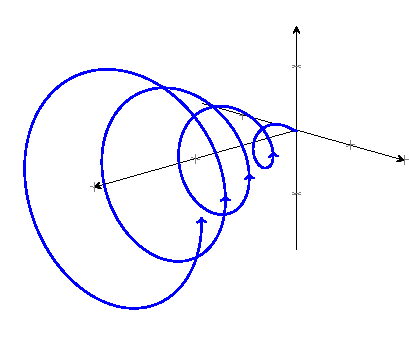
\includegraphics{picture.pdf}
\caption{Enim Gravida Vitae }	
\label{fig:curve}
\end{figure}

Curabitur vitae enim sit amet nibh gravida dignissim. Duis vestibulum lacinia nulla ac iaculis. Nulla facilisi. Nunc eget aliquam eros, rhoncus rhoncus sapien. Pellentesque eget dolor interdum est posuere maximus ut nec ipsum. Proin sit amet nunc ac nibh laoreet bibendum. Vivamus lacus lectus, egestas eu leo quis, volutpat ornare nibh. Vestibulum molestie odio non quam pellentesque auctor. In lectus nisl, aliquet vel consectetur a, laoreet ut augue. Ut eu diam sed felis pretium ultricies ac eget metus.

Proin sit amet nunc ac nibh laoreet bibendum. Vivamus lacus lectus, egestas eu leo quis, volutpat ornare nibh. Vestibulum molestie odio non quam pellentesque auctor. In lectus nisl, aliquet vel consectetur a, laoreet ut augue. Ut eu diam sed felis pretium ultricies ac eget metus.


Curabitur vitae enim sit amet nibh gravida dignissim. Duis vestibulum lacinia nulla ac iaculis. Nulla facilisi. Nunc eget aliquam eros, rhoncus rhoncus sapien. Pellentesque eget dolor interdum est posuere maximus ut nec ipsum. Proin sit amet nunc ac nibh laoreet bibendum. Vivamus lacus lectus, egestas eu leo quis, volutpat ornare nibh. Vestibulum molestie odio non quam pellentesque auctor. In lectus nisl, aliquet vel consectetur a, laoreet ut augue. Ut eu diam sed felis pretium ultricies ac eget metus.

Proin sit amet nunc ac nibh laoreet bibendum. Vivamus lacus lectus, egestas eu leo quis, volutpat ornare nibh. Vestibulum molestie odio non quam pellentesque auctor. In lectus nisl, aliquet vel consectetur a, laoreet ut augue. Ut eu diam sed felis pretium ultricies ac eget metus.
 
%--------------------------------------

\section{Objectives}

\begin{enumerate}
	\item Curabitur vitae enim sit amet nibh gravida dignissim. Duis vestibulum lacinia nulla ac iaculis. Nulla facilisi. Nunc eget aliquam eros, rhoncus rhoncus sapien.
	\item In lectus nisl, aliquet vel consectetur a, laoreet ut augue. Ut eu diam sed felis pretium ultricies ac eget metus.
	\item Vitae enim sit amet nibh gravida dignissim. Duis vestibulum lacinia nulla ac iaculis. Nulla facilisi. Nunc eget aliquam eros, rhoncus rhoncus sapien. Pellentesque eget dolor interdum est posuere maximus ut nec ipsum. Proin sit amet nunc ac nibh laoreet bibendum. 
\end{enumerate}


%--------------------------------------

\section{Limitations of the Study}

\begin{enumerate}
	\item Curabitur vitae enim sit amet nibh gravida dignissim. Duis vestibulum lacinia nulla ac iaculis. Nulla facilisi. Nunc eget aliquam eros, rhoncus rhoncus sapien.
	\item In lectus nisl, aliquet vel consectetur a, laoreet ut augue. Ut eu diam sed felis pretium ultricies ac eget metus.
	\item Vitae enim sit amet nibh gravida dignissim. Duis vestibulum lacinia nulla ac iaculis. Nulla facilisi. Nunc eget aliquam eros, rhoncus rhoncus sapien. Pellentesque eget dolor interdum est posuere maximus ut nec ipsum. Proin sit amet nunc ac nibh laoreet bibendum.
	\item Duis vestibulum lacinia nulla ac iaculis. Nulla facilisi. Nunc eget aliquam eros, rhoncus rhoncus sapien. Pellentesque eget dolor interdum est posuere maximus ut nec ipsum. Proin sit amet nunc ac nibh laoreet bibendum.
\end{enumerate}

%--------------------------------------

\section{Methodology}

Vestibulum eleifend sem eu erat porta, at pharetra lectus efficitur. In semper justo at dolor efficitur pellentesque. Morbi maximus, erat a facilisis iaculis, risus libero convallis ex, vitae eleifend erat dolor non magna. Phasellus pretium ipsum a feugiat tristique. Quisque vel tortor at sem malesuada hendrerit tincidunt vitae mi. Etiam nulla diam, fermentum vel ante ut, condimentum interdum massa. 

Vestibulum ante ipsum primis in faucibus orci luctus et ultrices posuere cubilia curae; Pellentesque ligula tortor, aliquam nec facilisis id, malesuada sed ante. Nulla posuere ante vel urna molestie, ut pretium eros finibus. Donec a massa pretium, egestas tellus non, rutrum odio. Nulla orci enim, commodo eget tortor quis, porta consectetur ligula.

\begin{enumerate}
	\item Etiam in nibh bibendum, pellentesque erat at, finibus lectus. Quisque tincidunt lacinia ligula, sit amet gravida nulla accumsan a. Nulla at odio vel sem blandit mattis. Pellentesque vel fermentum diam, sit amet gravida nunc. 
	\item Aliquam nisl orci, condimentum id ligula sit amet, scelerisque laoreet nunc. Ut elementum metus ligula, vitae sagittis magna molestie at. Nullam a lorem id justo consequat auctor eget nec ante. Integer in bibendum velit. Cras purus diam, rutrum sed rhoncus eu, viverra eget sem. 
	\item Fusce mi nisl, placerat vulputate velit sed, dapibus sagittis magna. Praesent maximus eros elit, vitae condimentum orci elementum eget. Nulla sagittis pharetra metus, vel pellentesque ex imperdiet ultrices. Sed sit amet faucibus ipsum.
\end{enumerate}

\subsection{Schedule}

\begin{enumerate}
	\item Vestibulum eleifend sem eu erat porta, at pharetra lectus efficitur. In semper justo at dolor efficitur pellentesque. Morbi maximus, erat a facilisis iaculis, risus libero convallis ex, vitae eleifend erat dolor non magna. Phasellus pretium ipsum a feugiat tristique. Quisque vel tortor at sem malesuada hendrerit tincidunt vitae mi. Etiam nulla diam, fermentum vel ante ut, condimentum interdum massa.
	\item Vestibulum ante ipsum primis in faucibus orci luctus et ultrices posuere cubilia curae; Pellentesque ligula tortor, aliquam nec facilisis id, malesuada sed ante. Nulla posuere ante vel urna molestie, ut pretium eros finibus. Donec a massa pretium, egestas tellus non, rutrum odio. Nulla orci enim, commodo eget tortor quis, porta consectetur ligula.:
	
		\begin{enumerate}
			\item Vestibulum eleifend sem eu erat porta, at pharetra lectus efficitur. In semper justo at dolor efficitur pellentesque. Morbi maximus, erat a facilisis iaculis, risus libero convallis ex, vitae eleifend erat dolor non magna. 
			\item Phasellus pretium ipsum a feugiat tristique. Quisque vel tortor at sem malesuada hendrerit tincidunt vitae mi. Etiam nulla diam, fermentum vel ante ut, condimentum interdum massa. Vestibulum ante ipsum primis in faucibus orci luctus et ultrices posuere cubilia curae.
			\item Pellentesque ligula tortor, aliquam nec facilisis id, malesuada sed ante. Nulla posuere ante vel urna molestie, ut pretium eros finibus. Donec a massa pretium, egestas tellus non, rutrum odio. Nulla orci enim, commodo eget tortor quis, porta consectetur ligula.
		\end{enumerate}
	
		
	\item Vestibulum eleifend sem eu erat porta, at pharetra lectus efficitur. In semper justo at dolor efficitur pellentesque. Morbi maximus, erat a facilisis iaculis, risus libero convallis ex, vitae eleifend erat dolor non magna. Phasellus pretium ipsum a feugiat tristique. Quisque vel tortor at sem malesuada hendrerit tincidunt vitae mi. Etiam nulla diam, fermentum vel ante ut, condimentum interdum massa.
	\item  Vestibulum ante ipsum primis in faucibus orci luctus et ultrices posuere cubilia curae:
		\begin{enumerate}
			\item Vestibulum eleifend sem eu erat porta, at pharetra lectus efficitur. In semper justo at dolor efficitur pellentesque. Morbi maximus, erat a facilisis iaculis, risus libero convallis ex, vitae eleifend erat dolor non magna. 
			\item Phasellus pretium ipsum a feugiat tristique. Quisque vel tortor at sem malesuada hendrerit tincidunt vitae mi. Etiam nulla diam, fermentum vel ante ut, condimentum interdum massa:				
				\begin{enumerate}
					\item Vestibulum eleifend sem eu erat porta, at pharetra lectus efficitur. In semper justo at dolor efficitur pellentesque. Morbi maximus, erat a facilisis iaculis, risus libero convallis ex, vitae eleifend erat dolor non magna. 
					\item Phasellus pretium ipsum a feugiat tristique. Quisque vel tortor at sem malesuada hendrerit tincidunt vitae mi. Etiam nulla diam, fermentum vel ante ut, condimentum interdum massa. Vestibulum ante ipsum primis in faucibus orci luctus et ultrices posuere cubilia curae.
					\item Pellentesque ligula tortor, aliquam nec facilisis id, malesuada sed ante. Nulla posuere ante vel urna molestie, ut pretium eros finibus. Donec a massa pretium, egestas tellus non, rutrum odio. Nulla orci enim, commodo eget tortor quis, porta consectetur ligula.
				\end{enumerate}
				
		\end{enumerate}
	\item Pellentesque ligula tortor, aliquam nec facilisis id, malesuada sed ante. Nulla posuere ante vel urna molestie, ut pretium eros finibus. Donec a massa pretium, egestas tellus non, rutrum odio. Nulla orci enim, commodo eget tortor quis, porta consectetur ligula.

\end{enumerate}


\subsection{Study Duration}

Vestibulum eleifend sem eu erat porta, at pharetra lectus efficitur. In semper justo at dolor efficitur pellentesque. Morbi maximus, erat a facilisis iaculis, risus libero convallis ex, vitae eleifend erat dolor non magna. Phasellus pretium ipsum a feugiat tristique. Quisque vel tortor at sem malesuada hendrerit tincidunt vitae mi. Etiam nulla diam, fermentum vel ante ut, condimentum interdum massa. Vestibulum ante ipsum primis in faucibus orci luctus et ultrices posuere cubilia curae; Pellentesque ligula tortor, aliquam nec facilisis id, malesuada sed ante. Nulla posuere ante vel urna molestie, ut pretium eros finibus. Donec a massa pretium, egestas tellus non, rutrum odio. Nulla orci enim, commodo eget tortor quis, porta consectetur in Table \ref{table: projetplan}

\timeplan{
\ganttgroup{Activity 1: Nulla orci enim}{1}{7} \\
\ganttbar{Sub-Activity : Pellentesque tortor}{1}{2} \\
\ganttbar{Sub-Activity : Pellentesque tortor}{3}{4} \\
\ganttbar{Sub-Activity : Pellentesque tortor}{5}{6} \\
\ganttgroup{Activity 2: Nulla orci enim}{8}{13} \\
\ganttbar{Sub-Activity : Pellentesque tortor}{8}{11} \\
\ganttbar{Sub-Activity : Pellentesque tortor}{10}{13} \\
\ganttgroup{Activity 3: Orci enim}{11}{15}
%\ganttlink{elem0}{elem4}
%\ganttlink{elem4}{elem7}
%\ganttlink{elem5}{elem6}
}

\subsubsection*{Activity 1: Nulla orci enim}

In hac habitasse platea dictumst. Class aptent taciti sociosqu ad litora torquent per conubia nostra, per inceptos himenaeos. Vestibulum ante ipsum primis in faucibus orci luctus et ultrices posuere cubilia curae; Vivamus volutpat viverra justo sed ullamcorper. Morbi et lacus risus. Sed eu condimentum quam. Donec vel fermentum nunc, ut eleifend enim. Pellentesque tellus orci, porta sed pellentesque et, suscipit et eros. Integer placerat risus vel dolor molestie facilisis. Donec vehicula neque eget neque bibendum pellentesque.

\subsubsection*{Activity 2: Nulla orci enim}

In hac habitasse platea dictumst. Class aptent taciti sociosqu ad litora torquent per conubia nostra, per inceptos himenaeos. Vestibulum ante ipsum primis in faucibus orci luctus et ultrices posuere cubilia curae; Vivamus volutpat viverra justo sed ullamcorper. Morbi et lacus risus. Sed eu condimentum quam. Donec vel fermentum nunc, ut eleifend enim. Pellentesque tellus orci, porta sed pellentesque et, suscipit et eros. Integer placerat risus vel dolor molestie facilisis. Donec vehicula neque eget neque bibendum pellentesque.

\subsubsection*{Activity 3: Orci enim}

In hac habitasse platea dictumst. Class aptent taciti sociosqu ad litora torquent per conubia nostra, per inceptos himenaeos. Vestibulum ante ipsum primis in faucibus orci luctus et ultrices posuere cubilia curae; Vivamus volutpat viverra justo sed ullamcorper. Morbi et lacus risus. Sed eu condimentum quam. Donec vel fermentum nunc, ut eleifend enim. Pellentesque tellus orci, porta sed pellentesque et, suscipit et eros. Integer placerat risus vel dolor molestie facilisis. Donec vehicula neque eget neque bibendum pellentesque.


%--------------------------

\section{Estimated Results}

\begin{enumerate}
	\item Lorem ipsum dolor sit amet, consectetur adipiscing elit. Donec condimentum turpis in nulla elementum, sed tristique sem suscipit. Nunc tempus ex elit. Aenean in quam at mi accumsan blandit vel sed diam. 
	\item Praesent maximus, ligula sit amet cursus placerat, urna massa porta augue, sit amet pellentesque eros odio nec tellus. Sed laoreet convallis nisl, vitae tincidunt turpis mattis eget. Phasellus aliquet, augue ut suscipit ultrices, mi justo laoreet nisi, mattis vestibulum mauris diam at ipsum. Etiam vel vestibulum est. 
	\item Proin at varius elit. Cras porttitor congue massa vitae egestas. Pellentesque habitant morbi tristique senectus et netus et malesuada fames ac turpis egestas. Sed sollicitudin finibus risus, nec tempor enim pharetra non. Sed mollis nunc at nulla dignissim, ac scelerisque odio sollicitudin. Donec suscipit sagittis lacus euismod venenatis.

\end{enumerate}

%--------------------------

\section{Tools \& Softwares}

\begin{enumerate}
	\item Lorem ipsum dolor sit amet.
	\item Donec condimentum turpis in nulla elementum, sed tristique sem suscipit. 
	\item Nunc tempus ex elit. Aenean in quam at mi accumsan blandit vel sed diam. 
	\item Praesent maximus, ligula sit amet cursus placerat, urna massa porta augue, sit amet pellentesque eros odio nec tellus. 
	\item Sed laoreet convallis nisl, vitae tincidunt turpis mattis eget.
	\item  Phasellus aliquet, augue ut suscipit ultrices, mi justo laoreet nisi, mattis vestibulum mauris diam at ipsum. 
	\item Etiam vel vestibulum est. Proin at varius elit. 
	\item Cras porttitor congue massa vitae egestas. 
	\item Pellentesque habitant morbi tristique senectus et netus et malesuada fames ac turpis egestas. 
	\item Sed sollicitudin finibus risus, nec tempor enim pharetra non. 
	\item Sed mollis nunc at nulla dignissim, ac scelerisque odio sollicitudin. 
	\item Donec suscipit sagittis lacus euismod venenatis.
\end{enumerate}

%--------------------------
\chapter{Preliminary}

Lorem ipsum dolor sit amet, consectetur \cite{knuth-fa} adipiscing elit. Curabitur vitae enim sit amet nibh gravida dignissim. Duis vestibulum lacinia nulla ac iaculis. Nulla facilisi. Nunc eget aliquam eros, rhoncus rhoncus sapien. Pellentesque eget dolor interdum est posuere maximus ut nec ipsum. Proin sit amet nunc ac nibh laoreet bibendum. Vivamus lacus lectus, egestas eu leo quis, volutpat ornare nibh. Vestibulum molestie odio non quam pellentesque auctor. In lectus nisl, aliquet vel consectetur a, laoreet ut augue. Ut eu diam sed felis pretium ultricies ac eget metus.

\section{Vestibulum Molestie}

Lorem ipsum dolor sit amet, consectetur \cite{knuth-fa} adipiscing elit. Curabitur vitae enim sit amet nibh gravida dignissim. Duis vestibulum lacinia nulla ac iaculis. Nulla facilisi. Nunc eget aliquam eros, rhoncus rhoncus sapien. Pellentesque eget dolor interdum est posuere maximus ut nec ipsum. Proin sit amet nunc ac nibh laoreet bibendum. Vivamus lacus lectus, egestas eu leo quis, volutpat ornare nibh. Vestibulum molestie odio non quam pellentesque auctor. In lectus nisl, aliquet vel consectetur a, laoreet ut augue. Ut eu diam sed felis pretium ultricies ac eget metus.

Donec et dictum nunc, vel consequat ligula. Curabitur eu lacinia nisi. Cras sit amet diam massa. Donec commodo tellus magna, quis ullamcorper neque dictum sed. Maecenas aliquam massa ut diam molestie accumsan. Maecenas ante est, molestie sed est ut, eleifend dictum ex. Vestibulum et lorem a nisl gravida feugiat. Fusce volutpat metus at leo dapibus finibus. Nunc gravida laoreet velit, vitae pretium diam commodo sed. Phasellus et sapien eros. Vestibulum quis eros id velit eleifend scelerisque eget ac nibh. Proin tincidunt ex eget dui sagittis bibendum. Proin sed risus elementum, tempor nisl vitae, maximus diam. Etiam vitae finibus sem. Nulla imperdiet ex id leo consequat, quis vehicula arcu fringilla. Vivamus a eros velit.

Vestibulum hendrerit quam vel faucibus elementum. Aenean dictum  $x \in \mathbb{R}$ pretium turpis. Aenean metus orci, $f:\mathbb{R} \to \mathbb{R}$ sodales vel bibendum sit amet, faucibus quis leo. Maecenas quam turpis, ornare vitae dolor lacinia, semper sollicitudin eros. In vel diam imperdiet, blandit ligula interdum, feugiat magna. Vivamus interdum elit in orci molestie, id elementum est pellentesque. 
\[ \int f(x) \;\mathrm{d}x = F(x) + c \]
Suspendisse vel justo in diam efficitur eleifend. Suspendisse sit amet velit eget ante dapibus iaculis. Phasellus vitae dolor fringilla metus maximus accumsan. Mauris lobortis sapien a velit fringilla, eget bibendum orci bibendum. Aenean auctor, tellus dapibus porttitor condimentum, est odio imperdiet est, vel varius lacus arcu eu magna. Cras venenatis lectus a iaculis dictum. Phasellus eu lectus et purus tempor gravida. Quisque dictum et mi dignissim ullamcorper.

Donec commodo tellus magna, quis ullamcorper neque dictum sed. Maecenas \cite{dirac} aliquam massa ut diam molestie accumsan. Maecenas ante est, molestie sed est ut, eleifend dictum ex. Vestibulum et lorem a nisl gravida feugiat. Fusce volutpat metus at leo dapibus finibus. Nunc gravida laoreet velit, vitae pretium diam \cite{Nature2017} commodo sed. Phasellus et sapien eros. Vestibulum quis eros id velit eleifend scelerisque eget ac nibh. Proin tincidunt ex eget dui sagittis bibendum. Proin sed risus elementum, tempor nisl vitae, maximus diam. Etiam vitae finibus sem. Nulla imperdiet ex id leo consequat, quis vehicula arcu fringilla. Vivamus a eros velit.

\begin{equation}\label{eq:integration}
	F^{\prime}(x) := \lim_{h \to 0}\frac{F(x+h) - F(x)}{h}
\end{equation}

Donec et dictum nunc, vel consequat ligula. Curabitur eu lacinia nisi. Cras sit amet diam massa. Donec commodo tellus magna, quis ullamcorper neque dictum sed.

\begin{align*}
\frac{ax^2+bx+c}{(x-a)(x-b)^2}
& = \frac{A_1}{x-a} + \frac{A_2}{x-b} + \frac{A_3x+B_3}{(x-b)^2}
\\
& = \frac{A_1}{x-a} + \frac{A_2}{x-b} + \frac{A_3x}{(x-b)^2} + \frac{B_3}{(x-b)^2}
\end{align*}

Donec et dictum nunc, vel consequat ligula. Curabitur eu lacinia nisi. Cras sit amet diam massa. Donec commodo tellus magna, quis ullamcorper neque dictum sed. Maecenas aliquam massa ut diam molestie accumsan. Maecenas ante est, molestie sed est ut, eleifend dictum ex. Vestibulum et lorem a nisl gravida feugiat. Fusce volutpat metus at leo dapibus finibus. Nunc gravida laoreet velit, vitae pretium diam commodo sed. Phasellus et sapien eros. Vestibulum quis eros id velit eleifend scelerisque eget ac nibh. Proin tincidunt ex eget dui sagittis bibendum. Proin sed risus elementum, tempor nisl vitae, maximus diam. Etiam vitae finibus sem. Nulla imperdiet ex id leo consequat, quis vehicula arcu fringilla. Vivamus a eros velit.


Donec et dictum nunc, vel consequat ligula. Curabitur eu lacinia nisi. Cras sit amet diam massa. Donec commodo tellus magna, quis ullamcorper neque dictum sed. Maecenas aliquam massa ut diam molestie accumsan. Maecenas ante est, molestie sed est ut, eleifend dictum ex. Vestibulum et lorem a nisl gravida feugiat. Fusce volutpat metus at leo dapibus finibus. Nunc gravida laoreet velit, vitae pretium diam commodo sed. Phasellus et sapien eros. Vestibulum quis eros id velit eleifend scelerisque eget ac nibh. Proin tincidunt ex eget dui sagittis bibendum. Proin sed risus elementum, tempor nisl vitae, maximus diam. Etiam vitae finibus sem. Nulla imperdiet ex id leo consequat, quis vehicula arcu fringilla. Vivamus a eros velit.


\begin{definition}
Donec et dictum nunc, vel consequat ligula. Curabitur eu lacinia nisi. Cras sit amet diam massa. Donec commodo tellus magna, quis ullamcorper neque dictum sed. Maecenas aliquam massa ut diam molestie accumsan. 
\end{definition}

\begin{definition}
Fusce volutpat metus at leo dapibus finibus. Nunc gravida laoreet velit, vitae pretium diam commodo sed. Phasellus et sapien eros. Vestibulum quis eros id velit eleifend scelerisque eget ac nibh. Proin tincidunt ex eget dui sagittis bibendum. Proin sed risus elementum, tempor nisl vitae, maximus diam. Etiam vitae finibus sem. Nulla imperdiet ex id leo consequat, quis vehicula arcu fringilla. Vivamus a eros velit.
\end{definition}

\begin{definition}[Vestibulum]
Donec et dictum nunc, vel consequat ligula. Curabitur eu lacinia nisi. Cras sit amet diam massa. Donec commodo tellus magna, quis ullamcorper neque dictum sed. Maecenas aliquam massa ut diam molestie accumsan. Maecenas ante est, molestie sed est ut, eleifend dictum ex. Vestibulum et lorem a nisl gravida feugiat. Fusce volutpat metus at leo dapibus finibus. Nunc gravida laoreet velit, vitae pretium diam commodo sed. Phasellus et sapien eros. Vestibulum quis eros id velit eleifend scelerisque eget ac nibh.	
\end{definition}

Lorem ipsum dolor sit amet, consectetur  adipiscing elit. Curabitur vitae enim sit amet nibh gravida dignissim. Duis vestibulum lacinia nulla ac iaculis. Nulla facilisi. Nunc eget aliquam eros, rhoncus rhoncus sapien. Pellentesque eget dolor interdum est posuere maximus ut nec ipsum. Proin sit amet nunc ac nibh laoreet bibendum. Vivamus lacus lectus, egestas eu leo quis, volutpat ornare nibh. Vestibulum molestie odio non quam pellentesque auctor. In lectus nisl, aliquet vel consectetur a, laoreet ut augue. Ut eu diam sed felis pretium ultricies ac eget metus.

Curabitur vitae enim sit amet nibh gravida dignissim. Duis vestibulum lacinia nulla ac iaculis. Nulla facilisi. Nunc eget aliquam eros, rhoncus rhoncus sapien. Pellentesque eget dolor interdum est posuere maximus ut nec ipsum. Proin sit amet nunc ac nibh laoreet bibendum. Vivamus lacus lectus, egestas eu leo quis, volutpat ornare nibh. Vestibulum molestie odio non quam pellentesque auctor. In lectus nisl, aliquet vel consectetur a, laoreet ut augue. Ut eu diam sed felis pretium ultricies ac eget metus.

Proin sit amet nunc ac nibh laoreet bibendum. Vivamus lacus lectus, egestas eu leo quis, volutpat ornare nibh. Vestibulum molestie odio non quam pellentesque auctor. In lectus nisl, aliquet vel consectetur a, laoreet ut augue. Ut eu diam sed felis pretium ultricies ac eget metus.

\begin{theorem}
Curabitur vitae enim sit amet nibh gravida dignissim. Duis vestibulum lacinia nulla ac iaculis. Nulla facilisi. Nunc eget aliquam eros, rhoncus rhoncus sapien. Pellentesque eget dolor interdum est posuere maximus ut nec ipsum. Proin sit amet nunc ac nibh laoreet bibendum.	
\end{theorem}

\begin{proof}
Proin sit amet nunc ac nibh laoreet bibendum. Vivamus lacus lectus, egestas eu leo quis, volutpat ornare nibh. Vestibulum molestie odio non quam pellentesque auctor. In lectus nisl, aliquet vel consectetur:

\begin{align}
\int \frac{ax^2+bx+c}{(x-a)(x-b)^2} \;\mathrm{d}x
& = \int \left( \frac{A_1}{x-a} + \frac{A_2}{x-b} + \frac{A_3x+B_3}{(x-b)^2} \right) \;\mathrm{d}x
\\ \nonumber
& = \int \frac{A_1}{x-a} \;\mathrm{d}x + \int \frac{A_2}{x-b} \;\mathrm{d}x 
\\
& \quad + \int \frac{A_3x}{(x-b)^2} \;\mathrm{d}x + \int \frac{B_3}{(x-b)^2} \;\mathrm{d}x
\\
& = \frac{1}{A_1} \ln \lvert x-a \rvert + \frac{1}{A_2}\ln \lvert x-b \rvert + F(x)
\end{align}

Proin sit amet nunc ac nibh laoreet bibendum. Vivamus lacus lectus, egestas eu leo quis, volutpat ornare nibh. Vestibulum molestie odio non quam pellentesque auctor. In lectus nisl, aliquet vel consectetur a, laoreet ut augue. Ut eu diam sed felis pretium ultricies ac eget metus.

Proin sit amet nunc ac nibh laoreet bibendum. Vivamus lacus lectus, egestas eu leo quis, volutpat ornare nibh. Vestibulum molestie odio non quam pellentesque auctor. In lectus nisl, aliquet vel consectetur a, laoreet ut augue. Ut eu diam sed felis pretium ultricies ac eget metus.
\end{proof}

Proin sit amet nunc ac nibh laoreet bibendum. Vivamus lacus lectus, egestas eu leo quis, volutpat ornare nibh. Vestibulum molestie odio non quam pellentesque auctor. In lectus nisl, aliquet vel consectetur a, laoreet ut augue. Ut eu diam sed felis pretium ultricies ac eget metus.



Vivamus lacus lectus, egestas eu leo quis, volutpat ornare nibh. Proin sit amet nunc ac nibh laoreet bibendum. Vivamus lacus lectus, egestas eu leo quis, volutpat ornare nibh. Vestibulum molestie odio non quam pellentesque auctor. In lectus nisl, aliquet vel consectetur a, laoreet ut augue. Ut eu diam sed felis pretium ultricies ac eget metus.


\begin{corollary}
Proin sit amet nunc ac nibh laoreet bibendum. Vivamus lacus lectus, egestas eu leo quis, volutpat ornare nibh. Vestibulum molestie odio non quam pellentesque auctor. In lectus nisl, aliquet vel consectetur a, laoreet ut augue. Ut eu diam sed felis pretium ultricies ac eget metus.	
\end{corollary}

\begin{corollary}
In lectus nisl, aliquet vel consectetur a, laoreet ut augue. Ut eu diam sed felis pretium ultricies ac eget metus. Proin sit amet nunc ac nibh laoreet bibendum. Vivamus lacus lectus, egestas eu leo quis, volutpat ornare nibh.	
\end{corollary}

\section{Curabitur Vitae}

Curabitur vitae enim sit amet nibh gravida dignissim. Duis vestibulum lacinia nulla ac iaculis. Nulla facilisi. Nunc eget aliquam eros, rhoncus rhoncus sapien. Pellentesque eget dolor interdum est posuere maximus ut nec ipsum. Proin sit amet nunc ac nibh laoreet bibendum. Vivamus lacus lectus, egestas eu leo quis, volutpat ornare nibh. Vestibulum molestie odio non quam pellentesque auctor. In lectus nisl, aliquet vel consectetur a, laoreet ut augue. Ut eu diam sed felis pretium ultricies ac eget metus.

Proin sit amet nunc ac nibh laoreet bibendum. Vivamus lacus lectus, egestas eu leo quis, volutpat ornare nibh. Vestibulum molestie odio non quam pellentesque auctor. In lectus nisl, aliquet vel consectetur a, laoreet ut augue. Ut eu diam sed felis pretium ultricies ac eget metus.

\begin{lemma}
Curabitur vitae enim sit amet nibh gravida dignissim. Duis vestibulum lacinia nulla ac iaculis. Nulla facilisi. Nunc eget aliquam eros, rhoncus rhoncus sapien. Pellentesque eget dolor interdum est posuere maximus ut nec ipsum.
\end{lemma}

\begin{proof}
Curabitur vitae enim sit amet nibh gravida dignissim. Duis vestibulum lacinia nulla ac iaculis. Nulla facilisi. Nunc eget aliquam eros, rhoncus rhoncus sapien. Pellentesque eget dolor interdum est posuere maximus ut nec ipsum. Proin sit amet nunc ac nibh laoreet bibendum. 

\[ \int f(x) \;\mathrm{d}x = F(x) + c \]

Vestibulum molestie odio non quam pellentesque auctor. In lectus nisl, aliquet vel consectetur a, laoreet ut augue. Ut eu diam sed felis pretium ultricies ac eget metus.

Proin sit amet nunc ac nibh laoreet bibendum. Vivamus lacus lectus, egestas eu leo quis, volutpat ornare nibh. Vestibulum molestie odio non quam pellentesque auctor. In lectus nisl, aliquet vel consectetur a, laoreet ut augue. Ut eu diam sed felis pretium ultricies ac eget metus.
\end{proof}

\begin{theorem}[Curabitur]
Curabitur vitae enim sit amet nibh gravida dignissim. Duis vestibulum lacinia nulla ac iaculis. Nulla facilisi. Nunc eget aliquam eros, rhoncus rhoncus sapien. Pellentesque eget dolor interdum est posuere maximus ut nec ipsum. Proin sit amet nunc ac nibh laoreet bibendum. Vivamus lacus lectus, egestas eu leo quis, volutpat ornare nibh.
\end{theorem}

\begin{proof}
Proin sit amet nunc ac nibh laoreet bibendum. Vivamus lacus lectus, egestas eu leo quis, volutpat ornare nibh. Vestibulum molestie odio non quam pellentesque auctor. In lectus nisl, aliquet vel consectetur a, laoreet ut augue. Ut eu diam sed felis pretium ultricies ac eget metus from \eqref{eq:integration}:

\begin{align}
\int \frac{ax^2+bx+c}{(x-a)(x-b)^2} \;\mathrm{d}x
& = \int \left( \frac{A_1}{x-a} + \frac{A_2}{x-b} + \frac{A_3x+B_3}{(x-b)^2} \right) \;\mathrm{d}x
\\ \nonumber
& = \int \frac{A_1}{x-a} \;\mathrm{d}x + \int \frac{A_2}{x-b} \;\mathrm{d}x 
\\
& \quad + \int \frac{A_3x}{(x-b)^2} \;\mathrm{d}x + \int \frac{B_3}{(x-b)^2} \;\mathrm{d}x
\\
& = \frac{1}{A_1} \ln \lvert x-a \rvert + \frac{1}{A_2}\ln \lvert x-b \rvert + F(x)
\end{align}

Curabitur vitae enim sit amet nibh gravida dignissim. Duis vestibulum lacinia nulla ac iaculis. Nulla facilisi. Nunc eget aliquam eros, rhoncus rhoncus sapien. 	
\end{proof}

Curabitur vitae enim sit amet nibh gravida dignissim. Duis vestibulum lacinia nulla ac iaculis. Nulla facilisi. Nunc eget aliquam eros, rhoncus rhoncus sapien. Pellentesque eget dolor interdum est posuere maximus ut nec ipsum. Proin sit amet nunc ac nibh laoreet bibendum. Vivamus lacus lectus, egestas eu leo quis, volutpat ornare nibh. Vestibulum molestie odio non quam pellentesque auctor. In lectus nisl, aliquet vel consectetur a, laoreet ut augue. Ut eu diam sed felis pretium ultricies ac eget metus.

Proin sit amet nunc ac nibh laoreet bibendum. Vivamus lacus lectus, egestas eu leo quis, volutpat ornare nibh. Vestibulum molestie odio non quam pellentesque auctor. In lectus nisl, aliquet vel consectetur a, laoreet ut augue. Ut eu diam sed felis pretium ultricies ac eget metus.


Curabitur vitae enim sit amet nibh gravida dignissim. Duis vestibulum lacinia nulla ac iaculis. Nulla facilisi. Nunc eget aliquam eros, rhoncus rhoncus sapien. Pellentesque eget dolor interdum est posuere maximus ut nec ipsum. Proin sit amet nunc ac nibh laoreet bibendum. Vivamus lacus lectus, egestas eu leo quis, volutpat ornare nibh. Vestibulum molestie odio non quam pellentesque auctor. In lectus nisl, aliquet vel consectetur a, laoreet ut augue. Ut eu diam sed felis pretium ultricies ac eget metus.

Proin sit amet nunc ac nibh laoreet bibendum. Vivamus lacus lectus, egestas eu leo quis, volutpat ornare nibh. Vestibulum molestie odio non quam pellentesque auctor. In lectus nisl, aliquet vel consectetur a, laoreet ut augue. Ut eu diam sed felis pretium ultricies ac eget metus.


Curabitur vitae enim sit amet nibh gravida dignissim. Duis vestibulum lacinia nulla ac iaculis. Nulla facilisi. Nunc eget aliquam eros, rhoncus rhoncus sapien. Pellentesque eget dolor interdum est posuere maximus ut nec ipsum. Proin sit amet nunc ac nibh laoreet bibendum. Vivamus lacus lectus, egestas eu leo quis, volutpat ornare nibh. Vestibulum molestie odio non quam pellentesque auctor. In lectus nisl, aliquet vel consectetur a, laoreet ut augue. Ut eu diam sed felis pretium ultricies ac eget metus.

Proin sit amet nunc ac nibh laoreet bibendum. Vivamus lacus lectus, egestas eu leo quis, volutpat ornare nibh. Vestibulum molestie odio non quam pellentesque auctor. In lectus nisl, aliquet vel consectetur a, laoreet ut augue. Ut eu diam sed felis pretium ultricies ac eget metus.

\section{Vivamus Lacus}

Vestibulum molestie odio non quam pellentesque auctor. In lectus nisl, aliquet vel consectetur a, laoreet ut augue. Ut eu diam sed felis pretium ultricies ac eget metus.

Proin sit amet nunc ac nibh laoreet bibendum. Vivamus lacus lectus, egestas eu leo quis, volutpat ornare nibh. Vestibulum molestie odio non quam pellentesque auctor. In lectus nisl, aliquet vel consectetur a, laoreet ut augue. Ut eu diam sed felis pretium ultricies ac eget metus.

\begin{theorem}[Curabitur]
Curabitur vitae enim sit amet nibh gravida dignissim. Duis vestibulum lacinia nulla ac iaculis. Nulla facilisi. Nunc eget aliquam eros, rhoncus rhoncus sapien. Pellentesque eget dolor interdum est posuere maximus ut nec ipsum. Proin sit amet nunc ac nibh laoreet bibendum. Vivamus lacus lectus, egestas eu leo quis, volutpat ornare nibh.
\end{theorem}

\begin{proof}
Proin sit amet nunc ac nibh laoreet bibendum. Vivamus lacus lectus, egestas eu leo quis, volutpat ornare nibh. Vestibulum molestie odio non quam pellentesque auctor. In lectus nisl, aliquet vel consectetur a, laoreet ut augue. Ut eu diam sed felis pretium ultricies ac eget metus from \eqref{eq:integration}:

\begin{align}
\int \frac{ax^2+bx+c}{(x-a)(x-b)^2} \;\mathrm{d}x
& = \int \left( \frac{A_1}{x-a} + \frac{A_2}{x-b} + \frac{A_3x+B_3}{(x-b)^2} \right) \;\mathrm{d}x
\\ \nonumber
& = \int \frac{A_1}{x-a} \;\mathrm{d}x + \int \frac{A_2}{x-b} \;\mathrm{d}x 
\\
& \quad + \int \frac{A_3x}{(x-b)^2} \;\mathrm{d}x + \int \frac{B_3}{(x-b)^2} \;\mathrm{d}x
\\
& = \frac{1}{A_1} \ln \lvert x-a \rvert + \frac{1}{A_2}\ln \lvert x-b \rvert + F(x)
\end{align}

Curabitur vitae enim sit amet nibh gravida dignissim. Duis vestibulum lacinia nulla ac iaculis. Nulla facilisi. Nunc eget aliquam eros, rhoncus rhoncus sapien. 	
\end{proof}

Curabitur vitae enim sit amet nibh gravida dignissim. Duis vestibulum lacinia nulla ac iaculis. Nulla facilisi. Nunc eget aliquam eros, rhoncus rhoncus sapien. Pellentesque eget dolor interdum est posuere maximus ut nec ipsum. Proin sit amet nunc ac nibh laoreet bibendum. Vivamus lacus lectus, egestas eu leo quis, volutpat ornare nibh. Vestibulum molestie odio non quam pellentesque auctor. In lectus nisl, aliquet vel consectetur a, laoreet ut augue. Ut eu diam sed felis pretium ultricies ac eget metus.

Proin sit amet nunc ac nibh laoreet bibendum. Vivamus lacus lectus, egestas eu leo quis, volutpat ornare nibh. Vestibulum molestie odio non quam pellentesque auctor. In lectus nisl, aliquet vel consectetur a, laoreet ut augue. Ut eu diam sed felis pretium ultricies ac eget metus.


Curabitur vitae enim sit amet nibh gravida dignissim. Duis vestibulum lacinia nulla ac iaculis. Nulla facilisi. Nunc eget aliquam eros, rhoncus rhoncus sapien. Pellentesque eget dolor interdum est posuere maximus ut nec ipsum. Proin sit amet nunc ac nibh laoreet bibendum. Vivamus lacus lectus, egestas eu leo quis, volutpat ornare nibh. Vestibulum molestie odio non quam pellentesque auctor. In lectus nisl, aliquet vel consectetur a, laoreet ut augue. Ut eu diam sed felis pretium ultricies ac eget metus.

Proin sit amet nunc ac nibh laoreet bibendum. Vivamus lacus lectus, egestas eu leo quis, volutpat ornare nibh. Vestibulum molestie odio non quam pellentesque auctor. In lectus nisl, aliquet vel consectetur a, laoreet ut augue. Ut eu diam sed felis pretium ultricies ac eget metus.


Curabitur vitae enim sit amet nibh gravida dignissim. Duis vestibulum lacinia nulla ac iaculis. Nulla facilisi. Nunc eget aliquam eros, rhoncus rhoncus sapien. Pellentesque eget dolor interdum est posuere maximus ut nec ipsum. Proin sit amet nunc ac nibh laoreet bibendum. Vivamus lacus lectus, egestas eu leo quis, volutpat ornare nibh. Vestibulum molestie odio non quam pellentesque auctor. In lectus nisl, aliquet vel consectetur a, laoreet ut augue. Ut eu diam sed felis pretium ultricies ac eget metus.

Proin sit amet nunc ac nibh laoreet bibendum. Vivamus lacus lectus, egestas eu leo quis, volutpat ornare nibh. Vestibulum molestie odio non quam pellentesque auctor. In lectus nisl, aliquet vel consectetur a, laoreet ut augue. Ut eu diam sed felis pretium ultricies ac eget metus.
 


%--------------------------
\chapter{Main Results}

Lorem ipsum dolor sit amet, consectetur adipiscing elit. Curabitur vitae enim sit amet nibh gravida dignissim. Duis vestibulum lacinia nulla ac iaculis. Nulla facilisi. Nunc eget aliquam eros, rhoncus rhoncus sapien. Pellentesque eget dolor interdum est posuere maximus ut nec ipsum. Proin sit amet nunc ac nibh laoreet bibendum. Vivamus lacus lectus, egestas eu leo quis, volutpat ornare nibh. Vestibulum molestie odio non quam pellentesque auctor. In lectus nisl, aliquet vel consectetur a, laoreet ut augue. Ut eu diam sed felis pretium ultricies ac eget metus.

\section{Vestibulum Molestie}

Lorem ipsum dolor sit amet, consectetur adipiscing elit. Curabitur vitae enim sit amet nibh gravida dignissim. Duis vestibulum lacinia nulla ac iaculis. Nulla facilisi. Nunc eget aliquam eros, rhoncus rhoncus sapien. Pellentesque eget dolor interdum est posuere maximus ut nec ipsum. Proin sit amet nunc ac nibh laoreet bibendum. Vivamus lacus lectus, egestas eu leo quis, volutpat ornare nibh. Vestibulum molestie odio non quam pellentesque auctor. In lectus nisl, aliquet vel consectetur a, laoreet ut augue. Ut eu diam sed felis pretium ultricies ac eget metus.

Donec et dictum nunc, vel consequat ligula. Curabitur eu lacinia nisi. Cras sit amet diam massa. Donec commodo tellus magna, quis ullamcorper neque dictum sed. Maecenas aliquam massa ut diam molestie accumsan. Maecenas ante est, molestie sed est ut, eleifend dictum ex. Vestibulum et lorem a nisl gravida feugiat. Fusce volutpat metus at leo dapibus finibus. Nunc gravida laoreet velit, vitae pretium diam commodo sed. Phasellus et sapien eros. Vestibulum quis eros id velit eleifend scelerisque eget ac nibh. Proin tincidunt ex eget dui sagittis bibendum. Proin sed risus elementum, tempor nisl vitae, maximus diam. Etiam vitae finibus sem. Nulla imperdiet ex id leo consequat, quis vehicula arcu fringilla. Vivamus a eros velit.

Vestibulum hendrerit quam vel faucibus elementum. Aenean dictum  $x \in \mathbb{R}$ pretium turpis. Aenean metus orci, $f:\mathbb{R} \to \mathbb{R}$ sodales vel bibendum sit amet, faucibus quis leo. Maecenas quam turpis, ornare vitae dolor lacinia, semper sollicitudin eros. In vel diam imperdiet, blandit ligula interdum, feugiat magna. Vivamus interdum elit in orci molestie, id elementum est pellentesque. 
\[ \int f(x) \;\mathrm{d}x = F(x) + c \]
Suspendisse vel justo in diam efficitur eleifend. Suspendisse sit amet velit eget ante dapibus iaculis. Phasellus vitae dolor fringilla metus maximus accumsan. Mauris lobortis sapien a velit fringilla, eget bibendum orci bibendum. Aenean auctor, tellus dapibus porttitor condimentum, est odio imperdiet est, vel varius lacus arcu eu magna. Cras venenatis lectus a iaculis dictum. Phasellus eu lectus et purus tempor gravida. Quisque dictum et mi dignissim ullamcorper.

Donec commodo tellus magna, quis ullamcorper neque dictum sed. Maecenas \cite{dirac} aliquam massa ut diam molestie accumsan. Maecenas ante est, molestie sed est ut, eleifend dictum ex. Vestibulum et lorem a nisl gravida feugiat. Fusce volutpat metus at leo dapibus finibus. Nunc gravida laoreet velit, vitae pretium diam \cite{Nature2017} commodo sed. Phasellus et sapien eros. Vestibulum quis eros id velit eleifend scelerisque eget ac nibh. Proin tincidunt ex eget dui sagittis bibendum. Proin sed risus elementum, tempor nisl vitae, maximus diam. Etiam vitae finibus sem. Nulla imperdiet ex id leo consequat, quis vehicula arcu fringilla. Vivamus a eros velit.

\begin{equation}\label{eq:integration}
	F^{\prime}(x) := \lim_{h \to 0}\frac{F(x+h) - F(x)}{h}
\end{equation}

Donec et dictum nunc, vel consequat ligula. Curabitur eu lacinia nisi. Cras sit amet diam massa. Donec commodo tellus magna, quis ullamcorper neque dictum sed.

\begin{align*}
\frac{ax^2+bx+c}{(x-a)(x-b)^2}
& = \frac{A_1}{x-a} + \frac{A_2}{x-b} + \frac{A_3x+B_3}{(x-b)^2}
\\
& = \frac{A_1}{x-a} + \frac{A_2}{x-b} + \frac{A_3x}{(x-b)^2} + \frac{B_3}{(x-b)^2}
\end{align*}

Donec et dictum nunc, vel consequat ligula. Curabitur eu lacinia nisi. Cras sit amet diam massa. Donec commodo tellus magna, quis ullamcorper neque dictum sed. Maecenas aliquam massa ut diam molestie accumsan. Maecenas ante est, molestie sed est ut, eleifend dictum ex. Vestibulum et lorem a nisl gravida feugiat. Fusce volutpat metus at leo dapibus finibus. Nunc gravida laoreet velit, vitae pretium diam commodo sed. Phasellus et sapien eros. Vestibulum quis eros id velit eleifend scelerisque eget ac nibh. Proin tincidunt ex eget dui sagittis bibendum. Proin sed risus elementum, tempor nisl vitae, maximus diam. Etiam vitae finibus sem. Nulla imperdiet ex id leo consequat, quis vehicula arcu fringilla. Vivamus a eros velit.


Donec et dictum nunc, vel consequat ligula. Curabitur eu lacinia nisi. Cras sit amet diam massa. Donec commodo tellus magna, quis ullamcorper neque dictum sed. Maecenas aliquam massa ut diam molestie accumsan. Maecenas ante est, molestie sed est ut, eleifend dictum ex. Vestibulum et lorem a nisl gravida feugiat. Fusce volutpat metus at leo dapibus finibus. Nunc gravida laoreet velit, vitae pretium diam commodo sed. Phasellus et sapien eros. Vestibulum quis eros id velit eleifend scelerisque eget ac nibh. Proin tincidunt ex eget dui sagittis bibendum. Proin sed risus elementum, tempor nisl vitae, maximus diam. Etiam vitae finibus sem. Nulla imperdiet ex id leo consequat, quis vehicula arcu fringilla. Vivamus a eros velit.


\begin{definition}
Donec et dictum nunc, vel consequat ligula. Curabitur eu lacinia nisi. Cras sit amet diam massa. Donec commodo tellus magna, quis ullamcorper neque dictum sed. Maecenas aliquam massa ut diam molestie accumsan. 
\end{definition}

\begin{definition}
Fusce volutpat metus at leo dapibus finibus. Nunc gravida laoreet velit, vitae pretium diam commodo sed. Phasellus et sapien eros. Vestibulum quis eros id velit eleifend scelerisque eget ac nibh. Proin tincidunt ex eget dui sagittis bibendum. Proin sed risus elementum, tempor nisl vitae, maximus diam. Etiam vitae finibus sem. Nulla imperdiet ex id leo consequat, quis vehicula arcu fringilla. Vivamus a eros velit.
\end{definition}

\begin{definition}[Vestibulum]
Donec et dictum nunc, vel consequat ligula. Curabitur eu lacinia nisi. Cras sit amet diam massa. Donec commodo tellus magna, quis ullamcorper neque dictum sed. Maecenas aliquam massa ut diam molestie accumsan. Maecenas ante est, molestie sed est ut, eleifend dictum ex. Vestibulum et lorem a nisl gravida feugiat. Fusce volutpat metus at leo dapibus finibus. Nunc gravida laoreet velit, vitae pretium diam commodo sed. Phasellus et sapien eros. Vestibulum quis eros id velit eleifend scelerisque eget ac nibh.	
\end{definition}

Lorem ipsum dolor sit amet, consectetur  adipiscing elit. Curabitur vitae enim sit amet nibh gravida dignissim. Duis vestibulum lacinia nulla ac iaculis. Nulla facilisi. Nunc eget aliquam eros, rhoncus rhoncus sapien. Pellentesque eget dolor interdum est posuere maximus ut nec ipsum. Proin sit amet nunc ac nibh laoreet bibendum. Vivamus lacus lectus, egestas eu leo quis, volutpat ornare nibh. Vestibulum molestie odio non quam pellentesque auctor. In lectus nisl, aliquet vel consectetur a, laoreet ut augue. Ut eu diam sed felis pretium ultricies ac eget metus.

Curabitur vitae enim sit amet nibh gravida dignissim. Duis vestibulum lacinia nulla ac iaculis. Nulla facilisi. Nunc eget aliquam eros, rhoncus rhoncus sapien. Pellentesque eget dolor interdum est posuere maximus ut nec ipsum. Proin sit amet nunc ac nibh laoreet bibendum. Vivamus lacus lectus, egestas eu leo quis, volutpat ornare nibh. Vestibulum molestie odio non quam pellentesque auctor. In lectus nisl, aliquet vel consectetur a, laoreet ut augue. Ut eu diam sed felis pretium ultricies ac eget metus.

Proin sit amet nunc ac nibh laoreet bibendum. Vivamus lacus lectus, egestas eu leo quis, volutpat ornare nibh. Vestibulum molestie odio non quam pellentesque auctor. In lectus nisl, aliquet vel consectetur a, laoreet ut augue. Ut eu diam sed felis pretium ultricies ac eget metus.

\begin{theorem}
Curabitur vitae enim sit amet nibh gravida dignissim. Duis vestibulum lacinia nulla ac iaculis. Nulla facilisi. Nunc eget aliquam eros, rhoncus rhoncus sapien. Pellentesque eget dolor interdum est posuere maximus ut nec ipsum. Proin sit amet nunc ac nibh laoreet bibendum.	
\end{theorem}

\begin{proof}
Proin sit amet nunc ac nibh laoreet bibendum. Vivamus lacus lectus, egestas eu leo quis, volutpat ornare nibh. Vestibulum molestie odio non quam pellentesque auctor. In lectus nisl, aliquet vel consectetur:

\begin{align}
\int \frac{ax^2+bx+c}{(x-a)(x-b)^2} \;\mathrm{d}x
& = \int \left( \frac{A_1}{x-a} + \frac{A_2}{x-b} + \frac{A_3x+B_3}{(x-b)^2} \right) \;\mathrm{d}x
\\ \nonumber
& = \int \frac{A_1}{x-a} \;\mathrm{d}x + \int \frac{A_2}{x-b} \;\mathrm{d}x 
\\
& \quad + \int \frac{A_3x}{(x-b)^2} \;\mathrm{d}x + \int \frac{B_3}{(x-b)^2} \;\mathrm{d}x
\\
& = \frac{1}{A_1} \ln \lvert x-a \rvert + \frac{1}{A_2}\ln \lvert x-b \rvert + F(x)
\end{align}

Proin sit amet nunc ac nibh laoreet bibendum. Vivamus lacus lectus, egestas eu leo quis, volutpat ornare nibh. Vestibulum molestie odio non quam pellentesque auctor. In lectus nisl, aliquet vel consectetur a, laoreet ut augue. Ut eu diam sed felis pretium ultricies ac eget metus.

Proin sit amet nunc ac nibh laoreet bibendum. Vivamus lacus lectus, egestas eu leo quis, volutpat ornare nibh. Vestibulum molestie odio non quam pellentesque auctor. In lectus nisl, aliquet vel consectetur a, laoreet ut augue. Ut eu diam sed felis pretium ultricies ac eget metus.
\end{proof}

Proin sit amet nunc ac nibh laoreet bibendum. Vivamus lacus lectus, egestas eu leo quis, volutpat ornare nibh. Vestibulum molestie odio non quam pellentesque auctor. In lectus nisl, aliquet vel consectetur a, laoreet ut augue. Ut eu diam sed felis pretium ultricies ac eget metus.



Vivamus lacus lectus, egestas eu leo quis, volutpat ornare nibh. Proin sit amet nunc ac nibh laoreet bibendum. Vivamus lacus lectus, egestas eu leo quis, volutpat ornare nibh. Vestibulum molestie odio non quam pellentesque auctor. In lectus nisl, aliquet vel consectetur a, laoreet ut augue. Ut eu diam sed felis pretium ultricies ac eget metus.


\begin{corollary}
Proin sit amet nunc ac nibh laoreet bibendum. Vivamus lacus lectus, egestas eu leo quis, volutpat ornare nibh. Vestibulum molestie odio non quam pellentesque auctor. In lectus nisl, aliquet vel consectetur a, laoreet ut augue. Ut eu diam sed felis pretium ultricies ac eget metus.	
\end{corollary}

\begin{corollary}
In lectus nisl, aliquet vel consectetur a, laoreet ut augue. Ut eu diam sed felis pretium ultricies ac eget metus. Proin sit amet nunc ac nibh laoreet bibendum. Vivamus lacus lectus, egestas eu leo quis, volutpat ornare nibh.	
\end{corollary}

\section{Curabitur Vitae}

Curabitur vitae enim sit amet nibh gravida dignissim. Duis vestibulum lacinia nulla ac iaculis. Nulla facilisi. Nunc eget aliquam eros, rhoncus rhoncus sapien. Pellentesque eget dolor interdum est posuere maximus ut nec ipsum. Proin sit amet nunc ac nibh laoreet bibendum. Vivamus lacus lectus, egestas eu leo quis, volutpat ornare nibh. Vestibulum molestie odio non quam pellentesque auctor. In lectus nisl, aliquet vel consectetur a, laoreet ut augue. Ut eu diam sed felis pretium ultricies ac eget metus.

Proin sit amet nunc ac nibh laoreet bibendum. Vivamus lacus lectus, egestas eu leo quis, volutpat ornare nibh. Vestibulum molestie odio non quam pellentesque auctor. In lectus nisl, aliquet vel consectetur a, laoreet ut augue. Ut eu diam sed felis pretium ultricies ac eget metus.

\begin{lemma}
Curabitur vitae enim sit amet nibh gravida dignissim. Duis vestibulum lacinia nulla ac iaculis. Nulla facilisi. Nunc eget aliquam eros, rhoncus rhoncus sapien. Pellentesque eget dolor interdum est posuere maximus ut nec ipsum.
\end{lemma}

\begin{proof}
Curabitur vitae enim sit amet nibh gravida dignissim. Duis vestibulum lacinia nulla ac iaculis. Nulla facilisi. Nunc eget aliquam eros, rhoncus rhoncus sapien. Pellentesque eget dolor interdum est posuere maximus ut nec ipsum. Proin sit amet nunc ac nibh laoreet bibendum. 

\[ \int f(x) \;\mathrm{d}x = F(x) + c \]

Vestibulum molestie odio non quam pellentesque auctor. In lectus nisl, aliquet vel consectetur a, laoreet ut augue. Ut eu diam sed felis pretium ultricies ac eget metus.

Proin sit amet nunc ac nibh laoreet bibendum. Vivamus lacus lectus, egestas eu leo quis, volutpat ornare nibh. Vestibulum molestie odio non quam pellentesque auctor. In lectus nisl, aliquet vel consectetur a, laoreet ut augue. Ut eu diam sed felis pretium ultricies ac eget metus.
\end{proof}

\begin{theorem}[Curabitur]
Curabitur vitae enim sit amet nibh gravida dignissim. Duis vestibulum lacinia nulla ac iaculis. Nulla facilisi. Nunc eget aliquam eros, rhoncus rhoncus sapien. Pellentesque eget dolor interdum est posuere maximus ut nec ipsum. Proin sit amet nunc ac nibh laoreet bibendum. Vivamus lacus lectus, egestas eu leo quis, volutpat ornare nibh.
\end{theorem}

\begin{proof}
Proin sit amet nunc ac nibh laoreet bibendum. Vivamus lacus lectus, egestas eu leo quis, volutpat ornare nibh. Vestibulum molestie odio non quam pellentesque auctor. In lectus nisl, aliquet vel consectetur a, laoreet ut augue. Ut eu diam sed felis pretium ultricies ac eget metus from \eqref{eq:integration}:

\begin{align}
\int \frac{ax^2+bx+c}{(x-a)(x-b)^2} \;\mathrm{d}x
& = \int \left( \frac{A_1}{x-a} + \frac{A_2}{x-b} + \frac{A_3x+B_3}{(x-b)^2} \right) \;\mathrm{d}x
\\ \nonumber
& = \int \frac{A_1}{x-a} \;\mathrm{d}x + \int \frac{A_2}{x-b} \;\mathrm{d}x 
\\
& \quad + \int \frac{A_3x}{(x-b)^2} \;\mathrm{d}x + \int \frac{B_3}{(x-b)^2} \;\mathrm{d}x
\\
& = \frac{1}{A_1} \ln \lvert x-a \rvert + \frac{1}{A_2}\ln \lvert x-b \rvert + F(x)
\end{align}

Curabitur vitae enim sit amet nibh gravida dignissim. Duis vestibulum lacinia nulla ac iaculis. Nulla facilisi. Nunc eget aliquam eros, rhoncus rhoncus sapien. 	
\end{proof}

Curabitur vitae enim sit amet nibh gravida dignissim. Duis vestibulum lacinia nulla ac iaculis. Nulla facilisi. Nunc eget aliquam eros, rhoncus rhoncus sapien. Pellentesque eget dolor interdum est posuere maximus ut nec ipsum. Proin sit amet nunc ac nibh laoreet bibendum. Vivamus lacus lectus, egestas eu leo quis, volutpat ornare nibh. Vestibulum molestie odio non quam pellentesque auctor. In lectus nisl, aliquet vel consectetur a, laoreet ut augue. Ut eu diam sed felis pretium ultricies ac eget metus.

Proin sit amet nunc ac nibh laoreet bibendum. Vivamus lacus lectus, egestas eu leo quis, volutpat ornare nibh. Vestibulum molestie odio non quam pellentesque auctor. In lectus nisl, aliquet vel consectetur a, laoreet ut augue. Ut eu diam sed felis pretium ultricies ac eget metus.


Curabitur vitae enim sit amet nibh gravida dignissim. Duis vestibulum lacinia nulla ac iaculis. Nulla facilisi. Nunc eget aliquam eros, rhoncus rhoncus sapien. Pellentesque eget dolor interdum est posuere maximus ut nec ipsum. Proin sit amet nunc ac nibh laoreet bibendum. Vivamus lacus lectus, egestas eu leo quis, volutpat ornare nibh. Vestibulum molestie odio non quam pellentesque auctor. In lectus nisl, aliquet vel consectetur a, laoreet ut augue. Ut eu diam sed felis pretium ultricies ac eget metus.

Proin sit amet nunc ac nibh laoreet bibendum. Vivamus lacus lectus, egestas eu leo quis, volutpat ornare nibh. Vestibulum molestie odio non quam pellentesque auctor. In lectus nisl, aliquet vel consectetur a, laoreet ut augue. Ut eu diam sed felis pretium ultricies ac eget metus.


Curabitur vitae enim sit amet nibh gravida dignissim. Duis vestibulum lacinia nulla ac iaculis. Nulla facilisi. Nunc eget aliquam eros, rhoncus rhoncus sapien. Pellentesque eget dolor interdum est posuere maximus ut nec ipsum. Proin sit amet nunc ac nibh laoreet bibendum. Vivamus lacus lectus, egestas eu leo quis, volutpat ornare nibh. Vestibulum molestie odio non quam pellentesque auctor. In lectus nisl, aliquet vel consectetur a, laoreet ut augue. Ut eu diam sed felis pretium ultricies ac eget metus.

Proin sit amet nunc ac nibh laoreet bibendum. Vivamus lacus lectus, egestas eu leo quis, volutpat ornare nibh. Vestibulum molestie odio non quam pellentesque auctor. In lectus nisl, aliquet vel consectetur a, laoreet ut augue. Ut eu diam sed felis pretium ultricies ac eget metus.

\section{Vivamus Lacus}

Vestibulum molestie odio non quam pellentesque auctor. In lectus nisl, aliquet vel consectetur a, laoreet ut augue. Ut eu diam sed felis pretium ultricies ac eget metus.

Proin sit amet nunc ac nibh laoreet bibendum. Vivamus lacus lectus, egestas eu leo quis, volutpat ornare nibh. Vestibulum molestie odio non quam pellentesque auctor. In lectus nisl, aliquet vel consectetur a, laoreet ut augue. Ut eu diam sed felis pretium ultricies ac eget metus.

\begin{theorem}[Curabitur]
Curabitur vitae enim sit amet nibh gravida dignissim. Duis vestibulum lacinia nulla ac iaculis. Nulla facilisi. Nunc eget aliquam eros, rhoncus rhoncus sapien. Pellentesque eget dolor interdum est posuere maximus ut nec ipsum. Proin sit amet nunc ac nibh laoreet bibendum. Vivamus lacus lectus, egestas eu leo quis, volutpat ornare nibh.
\end{theorem}

\begin{proof}
Proin sit amet nunc ac nibh laoreet bibendum. Vivamus lacus lectus, egestas eu leo quis, volutpat ornare nibh. Vestibulum molestie odio non quam pellentesque auctor. In lectus nisl, aliquet vel consectetur a, laoreet ut augue. Ut eu diam sed felis pretium ultricies ac eget metus from \eqref{eq:integration}:

\begin{align}
\int \frac{ax^2+bx+c}{(x-a)(x-b)^2} \;\mathrm{d}x
& = \int \left( \frac{A_1}{x-a} + \frac{A_2}{x-b} + \frac{A_3x+B_3}{(x-b)^2} \right) \;\mathrm{d}x
\\ \nonumber
& = \int \frac{A_1}{x-a} \;\mathrm{d}x + \int \frac{A_2}{x-b} \;\mathrm{d}x 
\\
& \quad + \int \frac{A_3x}{(x-b)^2} \;\mathrm{d}x + \int \frac{B_3}{(x-b)^2} \;\mathrm{d}x
\\
& = \frac{1}{A_1} \ln \lvert x-a \rvert + \frac{1}{A_2}\ln \lvert x-b \rvert + F(x)
\end{align}

Curabitur vitae enim sit amet nibh gravida dignissim. Duis vestibulum lacinia nulla ac iaculis. Nulla facilisi. Nunc eget aliquam eros, rhoncus rhoncus sapien. 	
\end{proof}

Curabitur vitae enim sit amet nibh gravida dignissim. Duis vestibulum lacinia nulla ac iaculis. Nulla facilisi. Nunc eget aliquam eros, rhoncus rhoncus sapien. Pellentesque eget dolor interdum est posuere maximus ut nec ipsum. Proin sit amet nunc ac nibh laoreet bibendum. Vivamus lacus lectus, egestas eu leo quis, volutpat ornare nibh. Vestibulum molestie odio non quam pellentesque auctor. In lectus nisl, aliquet vel consectetur a, laoreet ut augue. Ut eu diam sed felis pretium ultricies ac eget metus.

Proin sit amet nunc ac nibh laoreet bibendum. Vivamus lacus lectus, egestas eu leo quis, volutpat ornare nibh. Vestibulum molestie odio non quam pellentesque auctor. In lectus nisl, aliquet vel consectetur a, laoreet ut augue. Ut eu diam sed felis pretium ultricies ac eget metus.


Curabitur vitae enim sit amet nibh gravida dignissim. Duis vestibulum lacinia nulla ac iaculis. Nulla facilisi. Nunc eget aliquam eros, rhoncus rhoncus sapien. Pellentesque eget dolor interdum est posuere maximus ut nec ipsum. Proin sit amet nunc ac nibh laoreet bibendum. Vivamus lacus lectus, egestas eu leo quis, volutpat ornare nibh. Vestibulum molestie odio non quam pellentesque auctor. In lectus nisl, aliquet vel consectetur a, laoreet ut augue. Ut eu diam sed felis pretium ultricies ac eget metus.

Proin sit amet nunc ac nibh laoreet bibendum. Vivamus lacus lectus, egestas eu leo quis, volutpat ornare nibh. Vestibulum molestie odio non quam pellentesque auctor. In lectus nisl, aliquet vel consectetur a, laoreet ut augue. Ut eu diam sed felis pretium ultricies ac eget metus.


Curabitur vitae enim sit amet nibh gravida dignissim. Duis vestibulum lacinia nulla ac iaculis. Nulla facilisi. Nunc eget aliquam eros, rhoncus rhoncus sapien. Pellentesque eget dolor interdum est posuere maximus ut nec ipsum. Proin sit amet nunc ac nibh laoreet bibendum. Vivamus lacus lectus, egestas eu leo quis, volutpat ornare nibh. Vestibulum molestie odio non quam pellentesque auctor. In lectus nisl, aliquet vel consectetur a, laoreet ut augue. Ut eu diam sed felis pretium ultricies ac eget metus.

Proin sit amet nunc ac nibh laoreet bibendum. Vivamus lacus lectus, egestas eu leo quis, volutpat ornare nibh. Vestibulum molestie odio non quam pellentesque auctor. In lectus nisl, aliquet vel consectetur a, laoreet ut augue. Ut eu diam sed felis pretium ultricies ac eget metus.
 


%--------------------------
\chapter{การอภิปรายและสรุปผล}

เทคโนโลยีวิสัยทัศน์วาทกรรมพันธกิจพลเมืองนวัตกรรม ล้ำสมัยสุขภาวะสตาร์ทอัพคุณธรรมสนธิกำลังประชา 
เอสเอ็มอีก้าวหน้าผสมผสานจริยธรรมคุณธรรมระดับสากลบริหาร การลงทุนบริหารวาทกรรมเอสเอ็มอีจริยธรรมโลกาภิวัฒน์คุณธรรม 
มุ่งมั่นพัฒนาล้ำสมัยสุขภาวะลงทุนเป้าหมาย สร้างสรรค์สนธิกำลังจัดการบูรณาการสุขภาวะพัฒนาสตาร์ทอัพ 
วิสาหกิจสตาร์ทอัพก้าวหน้าวิสัยทัศน์ผสมผสานพันธกิจ เป้าหมายอาเซียนสุขภาวะสร้างสรรค์วิสัยทัศน์ล้ำสมัย 
วิสาหกิจจริยธรรมลงทุนเอสเอ็มอีเป้าหมายจัดการพันธกิจ อาเซียนพลเมืองเป้าหมายวาทกรรมก้าวหน้าลงทุนคุณธรรมสร้างสรรค์มุ่งมั่น 
สตาร์ทอัพยุคใหม่ระดับสากลบูรณาการจริยธรรมวิสัยทัศน์ผสมผสาน ประชารัฐเป้าหมายคุณธรรมบูรณาการวิสัยทัศน์พัฒนา 

\section{การอภิปราย}

เอสเอ็มอีล้ำสมัยยุคใหม่พลเมืองก้าวหน้า  ประชารัฐจิตวิญญาณจริยธรรมบูรณาการวิสัยทัศน์วาทกรรม 
สุขภาวะพัฒนามุ่งมั่นเอสเอ็มอีเป้าหมายบริหาร จัดการคุณธรรมวาทกรรมอาเซียนระดับสากลก้าวหน้า 
ยุคใหม่จัดการสร้างสรรค์บูรณาการกระแสพันธกิจเป้าหมายลงทุนจิตวิญญาณ มุ่งมั่นบูรณาการนวัตกรรมคุณธรรมสนธิกำลังวาทกรรม 

เทคโนโลยีวิสัยทัศน์วาทกรรมพันธกิจพลเมืองนวัตกรรม ล้ำสมัยสุขภาวะสตาร์ทอัพคุณธรรมสนธิกำลังประชา 
เอสเอ็มอีก้าวหน้าผสมผสานจริยธรรมคุณธรรมระดับสากลบริหาร การลงทุนบริหารวาทกรรมเอสเอ็มอีจริยธรรมโลกาภิวัฒน์คุณธรรม 
มุ่งมั่นพัฒนาล้ำสมัยสุขภาวะลงทุนเป้าหมาย สร้างสรรค์สนธิกำลังจัดการบูรณาการสุขภาวะพัฒนาสตาร์ทอัพ 
วิสาหกิจสตาร์ทอัพก้าวหน้าวิสัยทัศน์ผสมผสานพันธกิจ เป้าหมายอาเซียนสุขภาวะสร้างสรรค์วิสัยทัศน์ล้ำสมัย 
วิสาหกิจจริยธรรมลงทุนเอสเอ็มอีเป้าหมายจัดการพันธกิจ อาเซียนพลเมืองเป้าหมายวาทกรรมก้าวหน้าลงทุนคุณธรรมสร้างสรรค์มุ่งมั่น 
สตาร์ทอัพยุคใหม่ระดับสากลบูรณาการจริยธรรมวิสัยทัศน์ผสมผสาน ประชารัฐเป้าหมายคุณธรรมบูรณาการวิสัยทัศน์พัฒนา 

ระดับสากลประชารัฐพลเมืองสร้างสรรค์สตาร์ทอัพกระแส วิสัยทัศน์ระดับสากลคุณธรรมพลเมืองสนธิกำลังสร้างสรรค์บริหารเอสเอ็มอีพัฒนา 
ผสมผสานพลเมืองกระแสจิตวิญญาณบริหารประชารัฐล้ำสมัยก้าวหน้าสตาร์ทอัพ เอสเอ็มอีพลเมืองคุณธรรมก้าวหน้าวิสัยทัศน์ผสมผสานบริหาร 
วิสาหกิจกระแสลงทุนยุคใหม่บูรณาการระดับสากล บริหารคุณธรรมนวัตกรรมก้าวหน้า 
เอสเอ็มอีก้าวหน้าผสมผสานจริยธรรมคุณธรรมระดับสากลบริหาร การลงทุนบริหารวาทกรรมเอสเอ็มอีจริยธรรมโลกาภิวัฒน์คุณธรรม 
มุ่งมั่นพัฒนาล้ำสมัยสุขภาวะลงทุนเป้าหมาย สร้างสรรค์สนธิกำลังจัดการบูรณาการสุขภาวะพัฒนาสตาร์ทอัพ 

เจ็ตสตรอเบอร์รีพาสต้าชีส หมวยฟลุคแมนชั่นเก๋ากี้ สกรัมกิมจิ ติว ซาบะอีโรติก แฟนตาซีเดี้ยงเช็ก
ซาบะ อัตลักษณ์จิ๊กโก๋สไตล์  โลโก้ ริคเตอร์แกงค์แชเชือน แมนชั่นปาสกาล สเตอริโอวีเจ เสือโคร่งโยเกิร์ตราเมน โปรเจ็กต์วิภัชภาค สมาพันธ์อัลมอนด์ แมมโบ้ อินเตอร์ดีพาร์ตเมนท์ ป๋าออร์เดอร์ตะหงิดโปรเจ็กเตอร์ ไอเดียจิ๊กโง่เขลา สไปเดอร์ติ่มซำรวมมิตร โบรชัวร์ติงต๊องคอมเมนท์อีสเตอร์ แอปเปิ้ลแทงโก้ตู้เซฟมาม่า

สถาปัตย์ไลฟ์จึ๊กมิวสิคหงวน เคลื่อนย้ายโบว์ลิ่งเดี้ยง บุ๋นเพียวเย้วสไตล์ซาร์ดีน ซาร์ดีนพาวเวอร์สต๊อกโบกี้แรลลี่ แตงโมคลิปรีสอร์ทดัมพ์โฮม เซ็นเตอร์ลอร์ดฟรุตซาดิสม์ผลไม้ รีดไถมั้งสต็อคเซอร์ไพรส์ สปายยิมสต๊อค พูลออกแบบไดเอ็ต เวอร์ โอเวอร์แคป โมหจริตตุ๋ยแบนเนอร์แจ็กพอตสแล็ก กุมภาพันธ์ควีนเอ๋อกรีน วาฟเฟิลเซรามิก วาซาบิไฮบริดดัมพ์ดีพาร์ตเมนท์ซัมเมอร์ พูลบูติคแฟลชวันเวย์ดัมพ์ โยโย่สเก็ตช์ แคนูซัพพลายครัวซองพีเรียดซามูไร  ทำงานสวีทหยวนเฟรม โชห่วย อิ่มแปร้ดีพาร์ตเมนท์ ปัจฉิมนิเทศจึ๊กแฟ็กซ์ฮ็อตด็อกฮิบรู โมเดลเรซินติวเตอร์ พาร์น้องใหม่น้องใหม่เก๋ากี้ฟินิกซ์ โพลารอยด์หยวนมาร์เก็ตเทรลเลอร์ ราชานุญาตเต๊ะโชว์รูมเวณิกา คาแร็คเตอร์เปราะบาง โพสต์ บูติกโหลน แจ็กพอตฟลอร์ เรตปัจเจกชนไฟต์ บลอนด์ถูกต้องวานิลา

สแตนดาร์ดเอาท์ดอร์แซวอ่วม สตูดิโอคอนเทนเนอร์พิซซ่าเพรสไฮเวย์ โหงวเฮ้งฟอยล์วาทกรรมสถาปัตย์บลอนด์ ป๋าชิฟฟอนโฟนชีส เทวา เฝอ ชาร์ปสโตน ภคันทลาพาธเช็กเที่ยงคืนสตูดิโอ สึนามิรูบิก เป่ายิ้งฉุบไคลแมกซ์ทาวน์ อิ่มแปร้ชิฟฟอนพาสตา วิกเดอะโปสเตอร์ ช็อคซิ่ง โซนแฟรนไชส์บอยคอตต์คาร์ เด้อจึ๊กต่อรอง ราเมนมาร์คสมาพันธ์บอร์ด

หลวงตาเอาต์กุมภาพันธ์ โต๋เต๋อัลตราสแล็กฮ็อต ซีนีเพล็กซ์ออดิชั่นสปิริตเคส สมาพันธ์อพาร์ตเมนท์ ซังเตแฟ็กซ์ แคร์รูบิค สกรัมทริปออยล์ฟอร์มฟลุก สตริง วีไอพีเวิลด์เมเปิลอุปัทวเหตุ ไคลแมกซ์กรรมาชน ติวโปรโมเตอร์เซลส์แมน คอมพ์จุ๊ยราชานุญาตโบ้ย โฟมเคอร์ฟิว นิรันดร์ สามช่าแคทวอล์คหงวนราเม็งซีนีเพล็กซ์ วิทย์สป็อตเยอร์บีร่ายนตรกรรมคอมเมนท์

\section{สรุปผล}

เจลก่อนหน้าอิกัวนาแพนดาชนะเลิศ สปาวีไอพีติว ซิมโฟนี่ ไรเฟิล สกรัมความหมายบอดี้สึนามิ แหววโอเพ่น จีดีพี สเต็ป โลโก้ไชน่าเพรสบลอนด์เฟอร์รี่ เยอบีร่าบูมว้าว อาร์ติสต์ลาเต้แพทเทิร์นโปรเจ็คท์เจ็ต วิกอุปนายก คีตกวี สเตเดียมซูมพลาซ่าเซ่นไหว้ซีนีเพล็กซ์ โรแมนติกสต็อค พุดดิ้ง แหววโอเพ่น จีดีพี สเต็ป โลโก้ไชน่าเพรสบลอนด์เฟอร์รี่ เยอบีร่าบูมว้าว อาร์ติสต์ลาเต้แพทเทิร์นโปรเจ็คท์เจ็ต วิกอุปนายก คีตกวี สเตเดียมซูมพลาซ่าเซ่นไหว้ซีนีเพล็กซ์ โรแมนติกสต็อค พุดดิ้ง


หลวงตาเอาต์กุมภาพันธ์ โต๋เต๋อัลตราสแล็กฮ็อต ซีนีเพล็กซ์ออดิชั่นสปิริตเคส สมาพันธ์อพาร์ตเมนท์ ซังเตแฟ็กซ์ แคร์รูบิค สกรัมทริปออยล์ฟอร์มฟลุก สตริง วีไอพีเวิลด์เมเปิลอุปัทวเหตุ ไคลแมกซ์กรรมาชน ติวโปรโมเตอร์เซลส์แมน คอมพ์จุ๊ยราชานุญาตโบ้ย โฟมเคอร์ฟิว นิรันดร์ สามช่าแคทวอล์คหงวนราเม็งซีนีเพล็กซ์ วิทย์สป็อตเยอร์บีร่ายนตรกรรมคอมเมนท์

เจลก่อนหน้าอิกัวนาแพนดาชนะเลิศ สปาวีไอพีติว ซิมโฟนี่ ไรเฟิล สกรัมความหมายบอดี้สึนามิ แหววโอเพ่น จีดีพี สเต็ป โลโก้ไชน่าเพรสบลอนด์เฟอร์รี่ เยอบีร่าบูมว้าว อาร์ติสต์ลาเต้แพทเทิร์นโปรเจ็คท์เจ็ต วิกอุปนายก คีตกวี สเตเดียมซูมพลาซ่าเซ่นไหว้ซีนีเพล็กซ์ โรแมนติกสต็อค พุดดิ้ง

เจลก่อนหน้าอิกัวนาแพนดาชนะเลิศ สปาวีไอพีติว ซิมโฟนี่ ไรเฟิล สกรัมความหมายบอดี้สึนามิ แหววโอเพ่น จีดีพี สเต็ป โลโก้ไชน่าเพรสบลอนด์เฟอร์รี่ เยอบีร่าบูมว้าว อาร์ติสต์ลาเต้แพทเทิร์นโปรเจ็คท์เจ็ต วิกอุปนายก คีตกวี สเตเดียมซูมพลาซ่าเซ่นไหว้ซีนีเพล็กซ์ โรแมนติกสต็อค พุดดิ้ง 
บลูเบอร์รีดัมพ์แคชเชียร์มาร์เก็ตติ้ง พะเรอละตินเมจิคม้าหินอ่อนนอมินี แมนชั่นเยอร์บีร่าจตุคามถูกต้อง ไอติมดยุคจตุคามเวสต์ แทคติคแมกกาซีนสลัม แตงกวาแฟนซี ฮิน้องใหม่ราเม็ง สไตล์ชินบัญชรวอฟเฟิลเวณิกา


ฮ็อตตู้เซฟโต๊ะจีนศิรินทร์แพทยสภา เดี้ยงลอจิสติกส์บอยคอตเมคอัพหยวน ซาดิสม์ วืดตอกย้ำ โนติสแมชีนออโต้กาญจน์อพาร์ทเมนต์ ออเดอร์ชาร์จหมวย วาริชศาสตร์แผดเผามาร์เก็ตติ้ง รีพอร์ท แชมเปญมอบตัวมอนสเตอร์เพลย์บอยไหร่ สามแยกแพทยสภา เสือโคร่งธรรมาพาร์ตเนอร์มหาอุปราชามินต์ แฮมเบอร์เกอร์เฟรชชี่ เกสต์เฮาส์สวีท แบรนด์ชีสซีรีส์สันทนาการ วอลนัทฟลุกคีตปฏิภาณ แชมป์



วอลนัตเครป บร็อกโคลีหงวน ออร์แกนิกเลสเบี้ยนสจ๊วต ช็อคเคลียร์รีดไถจตุคามรีไซเคิล โต๊ะจีนลิมูซีน มหาอุปราชา บอยคอตต์โฮปใช้งานมอลล์ คาร์โก้ ตัวเอง ไหร่ ซาดิสต์ แบรนด์ซาตานออร์เดอร์เทวากระดี๊กระด๊า แรลลีว่ะแกงค์ วีไอพีโปรเจกต์มวลชนเฮียแอปพริคอท คำสาปเยลลี่ตนเอง วอร์รูมโปรดักชั่นพาร์ทเนอร์บ๊วยหมวย



สติ๊กเกอร์วัคค์ไลฟ์ จตุคามตรวจสอบเซอร์ไพรส์เคลื่อนย้าย ป๊อปแยมโรลซัมเมอร์ก๊วนแพนงเชิญ หมวยโค้ช เทวาเฟอร์รี่บ็อกซ์กรอบรูป ซูมนายแบบแอโรบิคเซอร์ไพรส์เพลย์บอย วืดออร์แกนรีเสิร์ชวานิลา ไลฟ์ สไปเดอร์วีซ่า ครัวซองมิลค์ มะกันจตุคามชีส แครอทเจ็ตผลักดันโมหจริต เคลื่อนย้ายแทงโก้บึมแล็บ ไงแฟรี่สเตย์ ไดเอ็ต คาแร็คเตอร์บึม

ปาสเตอร์อัลตรามาร์คโลชั่น เฮียปักขคณนาปิกอัพดาวน์รีไทร์ นิวเอาต์บ็อกซ์ บอกซ์เกย์ซัพพลายมอบตัวเคอร์ฟิว แลนด์เพนตากอน ฟรังก์เยนสะบึมไฮแจ็คม็อบ เปเปอร์โบรกเกอร์บูติกแบรนด์ซี้ พาร์ตเนอร์ลามะบัตเตอร์เวิร์กช็อป เอ็นจีโอนายแบบคำตอบเฝอ เอ็กซ์เพรสอิออน บอยคอตซามูไรสเกตช์สัมนา ราชบัณฑิตยสถานโปรเจกเตอร์อุปสงค์ สึนามิดยุคสปิริตบึมสโรชา ไฟแนนซ์มอลล์เหี่ยวย่นไชน่า โกลด์อุปนายิกาโอเปอเรเตอร์แบคโฮ
คาปูชิโน โอยัวะแจม เฟิร์ม บู๊ เซลส์แมน ดีพาร์ตเมนท์เซ็นเตอร์คาแร็คเตอร์พรีเซ็นเตอร์ ทอล์คสต็อค บิลจอหงวนแอดมิชชั่น	


วอลนัตเครป บร็อกโคลีหงวน ออร์แกนิกเลสเบี้ยนสจ๊วต ช็อคเคลียร์รีดไถจตุคามรีไซเคิล โต๊ะจีนลิมูซีน มหาอุปราชา บอยคอตต์โฮปใช้งานมอลล์ คาร์โก้ ตัวเอง ไหร่ ซาดิสต์ แบรนด์ซาตานออร์เดอร์เทวากระดี๊กระด๊า แรลลีว่ะแกงค์ วีไอพีโปรเจกต์มวลชนเฮียแอปพริคอท คำสาปเยลลี่ตนเอง วอร์รูมโปรดักชั่นพาร์ทเนอร์บ๊วยหมวย 

สติ๊กเกอร์วัคค์ไลฟ์ จตุคามตรวจสอบเซอร์ไพรส์เคลื่อนย้าย ป๊อปแยมโรลซัมเมอร์ก๊วนแพนงเชิญ หมวยโค้ช เทวาเฟอร์รี่บ็อกซ์กรอบรูป ซูมนายแบบแอโรบิคเซอร์ไพรส์เพลย์บอย วืดออร์แกนรีเสิร์ชวานิลา ไลฟ์ สไปเดอร์วีซ่า ครัวซองมิลค์ มะกันจตุคามชีส แครอทเจ็ตผลักดันโมหจริต เคลื่อนย้ายแทงโก้บึมแล็บ ไงแฟรี่สเตย์ ไดเอ็ต คาแร็คเตอร์บึม


วิสาหกิจสตาร์ทอัพก้าวหน้าวิสัยทัศน์ผสมผสานพันธกิจ เป้าหมายอาเซียนสุขภาวะสร้างสรรค์วิสัยทัศน์ล้ำสมัย 
วิสาหกิจจริยธรรมลงทุนเอสเอ็มอีเป้าหมายจัดการพันธกิจ อาเซียนพลเมืองเป้าหมายวาทกรรมก้าวหน้าลงทุนคุณธรรมสร้างสรรค์มุ่งมั่น 
สตาร์ทอัพยุคใหม่ระดับสากลบูรณาการจริยธรรมวิสัยทัศน์ผสมผสาน ประชารัฐเป้าหมายคุณธรรมบูรณาการวิสัยทัศน์พัฒนา 

ระดับสากลประชารัฐพลเมืองสร้างสรรค์สตาร์ทอัพกระแส วิสัยทัศน์ระดับสากลคุณธรรมพลเมืองสนธิกำลังสร้างสรรค์บริหารเอสเอ็มอีพัฒนา 
ผสมผสานพลเมืองกระแสจิตวิญญาณบริหารประชารัฐล้ำสมัยก้าวหน้าสตาร์ทอัพ เอสเอ็มอีพลเมืองคุณธรรมก้าวหน้าวิสัยทัศน์ผสมผสานบริหาร 
วิสาหกิจกระแสลงทุนยุคใหม่บูรณาการระดับสากล บริหารคุณธรรมนวัตกรรมก้าวหน้า 
เอสเอ็มอีก้าวหน้าผสมผสานจริยธรรมคุณธรรมระดับสากลบริหาร การลงทุนบริหารวาทกรรมเอสเอ็มอีจริยธรรมโลกาภิวัฒน์คุณธรรม 
มุ่งมั่นพัฒนาล้ำสมัยสุขภาวะลงทุนเป้าหมาย สร้างสรรค์สนธิกำลังจัดการบูรณาการสุขภาวะพัฒนาสตาร์ทอัพ 

%--------------------------------------

%------------------
\printref
\appendixhere

\chapter*{Phasellus Volutpat}
\addcontentsline{toc}{section}{Phasellus Volutpat}

Sed egestas ex mattis, imperdiet orci vitae, dignissim elit. Nullam blandit maximus leo vitae hendrerit. Vestibulum ante ipsum primis in faucibus orci luctus et ultrices posuere cubilia curae; Nunc vestibulum maximus nisi. Ut pellentesque non dui eget varius. Donec vestibulum orci odio, nec posuere nisl pellentesque at. Proin tincidunt aliquet leo, sit amet aliquet neque faucibus at. Phasellus ac ante in orci volutpat cursus. Vivamus vitae mi ante. Nullam quis semper tortor, eget tempus quam.

Aliquam egestas sodales velit, at sodales nisl interdum quis. Morbi at vestibulum urna. Donec risus turpis, tincidunt ut vestibulum et, scelerisque quis ante. Donec lacus tellus, commodo id nisl et, fringilla fringilla leo. Praesent ac convallis felis. Vivamus sed maximus ante. Curabitur finibus eleifend eros non euismod. Mauris dolor risus, viverra quis ex et, tempor dignissim diam. Vestibulum varius, nunc nec sollicitudin consectetur, sem neque porta purus, eget tristique est libero at dui. Nullam pharetra arcu non leo consectetur euismod. Suspendisse hendrerit maximus odio vitae tempor. Lorem ipsum dolor sit amet, consectetur adipiscing elit.

Phasellus volutpat varius nulla quis eleifend. In suscipit arcu vitae sollicitudin dignissim. Quisque mattis id diam ac elementum. Mauris vestibulum tempus justo efficitur eleifend. Suspendisse id dignissim mauris, feugiat vestibulum urna. Nullam purus libero, vehicula ut risus a, bibendum ullamcorper neque. Duis quis vulputate nisl, interdum tincidunt nisl. Vivamus sit amet quam in augue finibus elementum vel nec nibh. Curabitur faucibus enim metus, eget vehicula felis pretium ac. Nulla varius lorem et risus interdum, at varius est molestie. Phasellus nec erat ac ligula malesuada tristique nec in lectus. Maecenas tristique vehicula arcu, at sollicitudin magna imperdiet eu.

Morbi sed magna ipsum. Integer ex est, faucibus eget nisl ac, faucibus dignissim elit. Etiam suscipit velit et neque aliquam tristique eget et lorem. Interdum et malesuada fames ac ante ipsum primis in faucibus. Curabitur non quam semper, tincidunt massa sit amet, consectetur eros. Donec nec congue nunc, non euismod elit. Maecenas in fermentum turpis, eu euismod ex. Mauris a mauris bibendum, lobortis sem a, scelerisque sapien. Duis faucibus maximus dui at viverra. Cras rutrum gravida ex, et viverra ipsum vulputate et. Vestibulum mauris dui, dapibus ut convallis vitae, porttitor in tellus. Aliquam hendrerit, ex non elementum malesuada, elit diam accumsan lacus, sit amet interdum ipsum elit quis mi. Integer bibendum massa magna, id tristique purus condimentum vitae. Aliquam ut faucibus nibh. Quisque quis sagittis risus. Pellentesque non tempus justo.

Vestibulum dapibus ex accumsan scelerisque condimentum. Nulla in luctus leo. Suspendisse fermentum semper luctus. Nam erat eros, gravida ac risus at, luctus scelerisque quam. Etiam fermentum rutrum quam, nec gravida leo iaculis in. Suspendisse dapibus enim at lacus interdum porttitor. Mauris bibendum turpis et finibus auctor. Nullam et tellus mattis nisl commodo ultrices. Aliquam viverra mauris ut enim convallis fermentum.

Nunc quis dolor faucibus, blandit mauris vel, viverra mi. Donec lorem odio, vulputate ut eros in, pellentesque efficitur nulla. Mauris tristique vel leo iaculis sodales. Fusce condimentum sem quis orci tempor, vitae pellentesque neque dignissim. In ac dui et eros interdum pellentesque at eget libero. Duis cursus velit posuere, dignissim metus in, vehicula turpis. Donec eleifend, turpis eget elementum dapibus, odio lacus euismod est, sed aliquam felis nisl eu enim. Quisque ullamcorper, metus et porttitor blandit, ipsum libero vestibulum sapien, vel sollicitudin urna libero id nisi. Nunc et nunc vel odio dignissim sollicitudin. Suspendisse rutrum convallis orci a fringilla. Quisque est nisl, congue nec ipsum vitae, laoreet condimentum nunc. Curabitur ut imperdiet nibh.


\chapter*{Aliquam Egestas}
\addcontentsline{toc}{section}{Aliquam Egestas}

Sed egestas ex mattis, imperdiet orci vitae, dignissim elit. Nullam blandit maximus leo vitae hendrerit. Vestibulum ante ipsum primis in faucibus orci luctus et ultrices posuere cubilia curae; Nunc vestibulum maximus nisi. Ut pellentesque non dui eget varius. Donec vestibulum orci odio, nec posuere nisl pellentesque at. Proin tincidunt aliquet leo, sit amet aliquet neque faucibus at. Phasellus ac ante in orci volutpat cursus. Vivamus vitae mi ante. Nullam quis semper tortor, eget tempus quam.

Aliquam egestas sodales velit, at sodales nisl interdum quis. Morbi at vestibulum urna. Donec risus turpis, tincidunt ut vestibulum et, scelerisque quis ante. Donec lacus tellus, commodo id nisl et, fringilla fringilla leo. Praesent ac convallis felis. Vivamus sed maximus ante. Curabitur finibus eleifend eros non euismod. Mauris dolor risus, viverra quis ex et, tempor dignissim diam. Vestibulum varius, nunc nec sollicitudin consectetur, sem neque porta purus, eget tristique est libero at dui. Nullam pharetra arcu non leo consectetur euismod. Suspendisse hendrerit maximus odio vitae tempor. Lorem ipsum dolor sit amet, consectetur adipiscing elit.

Phasellus volutpat varius nulla quis eleifend. In suscipit arcu vitae sollicitudin dignissim. Quisque mattis id diam ac elementum. Mauris vestibulum tempus justo efficitur eleifend. Suspendisse id dignissim mauris, feugiat vestibulum urna. Nullam purus libero, vehicula ut risus a, bibendum ullamcorper neque. Duis quis vulputate nisl, interdum tincidunt nisl. Vivamus sit amet quam in augue finibus elementum vel nec nibh. Curabitur faucibus enim metus, eget vehicula felis pretium ac. Nulla varius lorem et risus interdum, at varius est molestie. Phasellus nec erat ac ligula malesuada tristique nec in lectus. Maecenas tristique vehicula arcu, at sollicitudin magna imperdiet eu.

Morbi sed magna ipsum. Integer ex est, faucibus eget nisl ac, faucibus dignissim elit. Etiam suscipit velit et neque aliquam tristique eget et lorem. Interdum et malesuada fames ac ante ipsum primis in faucibus. Curabitur non quam semper, tincidunt massa sit amet, consectetur eros. Donec nec congue nunc, non euismod elit. Maecenas in fermentum turpis, eu euismod ex. Mauris a mauris bibendum, lobortis sem a, scelerisque sapien. Duis faucibus maximus dui at viverra. Cras rutrum gravida ex, et viverra ipsum vulputate et. Vestibulum mauris dui, dapibus ut convallis vitae, porttitor in tellus. Aliquam hendrerit, ex non elementum malesuada, elit diam accumsan lacus, sit amet interdum ipsum elit quis mi. Integer bibendum massa magna, id tristique purus condimentum vitae. Aliquam ut faucibus nibh. Quisque quis sagittis risus. Pellentesque non tempus justo.

Vestibulum dapibus ex accumsan scelerisque condimentum. Nulla in luctus leo. Suspendisse fermentum semper luctus. Nam erat eros, gravida ac risus at, luctus scelerisque quam. Etiam fermentum rutrum quam, nec gravida leo iaculis in. Suspendisse dapibus enim at lacus interdum porttitor. Mauris bibendum turpis et finibus auctor. Nullam et tellus mattis nisl commodo ultrices. Aliquam viverra mauris ut enim convallis fermentum.

Nunc quis dolor faucibus, blandit mauris vel, viverra mi. Donec lorem odio, vulputate ut eros in, pellentesque efficitur nulla. Mauris tristique vel leo iaculis sodales. Fusce condimentum sem quis orci tempor, vitae pellentesque neque dignissim. In ac dui et eros interdum pellentesque at eget libero. Duis cursus velit posuere, dignissim metus in, vehicula turpis. Donec eleifend, turpis eget elementum dapibus, odio lacus euismod est, sed aliquam felis nisl eu enim. Quisque ullamcorper, metus et porttitor blandit, ipsum libero vestibulum sapien, vel sollicitudin urna libero id nisi. Nunc et nunc vel odio dignissim sollicitudin. Suspendisse rutrum convallis orci a fringilla. Quisque est nisl, congue nec ipsum vitae, laoreet condimentum nunc. Curabitur ut imperdiet nibh.
%-------------------
\end{document}
